%
% Szablon, v. 3.0
% p.wlaz@pollub.pl
%

% PROSZĘ NIE USUWAĆ
% KOMENTARZY Z~PREAMBUŁY
% JEŻELI KTOŚ WAM WMAWIA, ŻE
% TO PRZYSPIESZY COKOLWIEK
% -- MYLI SIĘ!


\documentclass[12pt]{mwbk}


%%%%%%% marinesy, rozmiary, to warto dopasować do drukarki
\usepackage[a4paper,twoside,top=2.6cm,bottom=2.6cm,inner=3cm,outer=2.6cm]{geometry}

%%%%%%%% polszczyzna
\usepackage[T1]{polski}


%%%%%%%%% sposób kodowania literek w edytorze
\usepackage[utf8]{inputenc}

\usepackage[font=small,labelfont=bf,justification=centering]{caption}


%%%% gdyby ktoś chciał powyklejać z~pedeefa
%%%% teksty za pomocą AcroReadera, to 
%%%% poniższe dwie linijki pomogą w~tym
%%%% Może to być przydatne, gdyby ktoś na podstawie
%%%% elektronicznej wersji chciał przygotować dane do 
%%%% badania antyplagiatowego
%%%% ponieważ prace są w
%%%% tych czasach różnymi
%%%% programami antyplagiatowymi
%%%% proszę absolutni NIE
%%%% USUWAĆ następujących
%%%% dwu linijek
\input glyphtounicode.tex
\pdfgentounicode = 1

%%%%%%%%%%%%%%%%%%%%%%%%%%%%%%%%%%%%%
%%%%% jeśli chcesz by główny tekst oraz wzory matematyczne były
%%%%% składane czcionką typu Times Roman (w~odróżnieniu od standardowej
%%%%% TeXowej, czyli Computer Modern Roman) to linia poniżej
%%%%% ma być 'aktywna', następna nieaktywna, 
%%%%% jeśli zrobisz odwrotnie (pierwsza nieaktywna,
%%%%% druga aktywna) uzyskasz skład czcionką
%%%%% Computer Modern Roman mającą wielu wiernych
%%%%% fanów w~świecie TeXa). Konsekwencją jednak będą zmiany
%%%%% rozmiarów czcionek dla rozdziałó i podrozdziałów - rzecz bez większego
%%%%% znaczenia, wynikająca z pewnych zaszłości historycznych (ComputerModern
%%%%% niegdyś były używane wyłącznie w postaci tzw. bitmap)
\usepackage{mathptmx} \usepackage{tgtermes}
%\usepackage{lmodern}

%%% WSZELKIE ZMIANY W~PREAMBULE RÓB ROZWAŻNIE
%%% NIE JESTEŚ PEWNY/PEWNA ICH EFEKTU TO~SPRAWDŹ 
%%% CZY W~PRGRAMIE ADOBE READER (i~to dokładnie
%%% o~ten program chodzi, nie o~jakikolwiek)
%%% Z~WYNIKOWEGO PLIU PDF DA SIE PRAWIDŁOWO
%%% WYKLEIĆ TEKST Z~POLSKIMI LITERAMI, BEZ KRZAKÓW,
%%%% BEZ DZIWACTW.


%%%%%%%%%%%%%% pozostałe pakiety używane w~pracy, to już zależy od
%%%%%%%%%%%%%% autora, więc może być tego więcej
\usepackage{fancyhdr}
\usepackage{graphicx}
\usepackage{amsmath}
\usepackage{amsthm}
\usepackage{amssymb}
\usepackage{url}
\usepackage{longtable}
\usepackage{array,hhline}

%%%%%%%% hyperref po to by przeglądarka pedeef ukazywala na odwołania
%%%%%%%% prawidłowo skonstruowane za pomocą \ref, \cite i.t.d. jako
%%%%%%%% hiperłącza
\usepackage{hyperref}



%%%%% dla fanów ``profesjonalnych'' tabel w~stylu zachodnich książek

\usepackage{booktabs} \heavyrulewidth=1.5bp \lightrulewidth=0.5bp


%%%%%%%%%%% poniżej uniwersalny sposób na ucywilizowanie znaków 
%%%%%%%%%%% niewiększości, niezależny od pakietu {polski}, ale za to 
%%%%%%%%%%% zależny od {amssymb}, ma tą zaletę, że działa np. z Timesem
%%%%%%%%%%% w matematyce
\let\leq\leqslant\let\le\leq\let\geq\geqslant\let\ge\geq


%%%%%%% jeżeli będziesz chciał włączać do swojej pracy fragmenty programów, 
%% to ponizsza linijka przyda się, jeśli nie - usuń ją

\usepackage{fancyvrb}


%%%%%%%%%%%%%%%%% struktury do tworzenia twierdzeń i~tym podobnych

\theoremstyle{plain}
\newtheorem{twier}{Twierdzenie}[chapter] % pierwsze to nazwa środowiska,
                                      %drugie to wyświetlana nazwa
				% to trzecie w~nawiasie kwadratowym
				% wskazuje numer dolepiony z~lewej do
				% numeru twierdzenia (tu numer
				% 'chapter', 
\newtheorem{lemat}{Lemat}[chapter]

\theoremstyle{definition}
\newtheorem{defi}{Definicja}[chapter]

\theoremstyle{remark}
\newtheorem{uwaga}{Uwaga}[chapter]
\newtheorem{wniosek}{Wniosek}[chapter]

%%%%% więcej możliwości w~dokumentacji amsthm



%%%%%%%%%%%%%%%%%%%%%%%%%%%%%%%%%%%%%%%%%5
%%%%%%%%%%%%%%%%%%%%%%%%%%%%%%%%%%%%%%%%%%
%%%%%%%%% wcięcie akapitowe %%%%%%%%%%%%%%
%%%%%%%%%%%%%%%%%%%%%%%%%%%%%%%%%%%%%%%%%%
%%%%%% ustawić w~zaleceń i~gustu %%%%%%%%%
%%%%%%%%%%%%%%%%%%%%%%%%%%%%%%%%%%%%%%%%%%
%%%%%%%% zalecenie na stronie wydziałowej
%%%%%%%% było 1.25cm i wyglądało jakoś 
%%%%%%%% śmiesznie duże, więc spłoszony nieco
%%%%%%%% wpisałem 1cm, ale uważny czytelnik już
%%%%%%%% zapewne się domyśli, że podmiana napisu 
%%%%%%%% =1cm na =1.25cm sprawi, że wcięcia na początku
%%%%%%%% akapitu ustawią się na (nieco przydużą)
%%%%%%%% wartość 1.25cm 

\parindent=1cm



%%%%%%%%%%%%%%%%%%%%%%%%%%%%%%%%
%%%%% tu pewne poluzowanie rozmieszczenia elementów tabelek
%%%%% możecie sobie poeksperymentować, by dopasować do swych
%%%%% gustów, a przede wszystkim gustów promotorów (promotorek)
  \tabcolsep=4mm          
  %\renewcommand\arraystretch{1.3}
%%%%%%%%%%%%%%%%%%%%%%%%%%%%%%%%%%



%%%%%%%%% teraz żywa pagina (aka 'running headline') i~numerowanie stron
%%%%%%%%%%%%%%%%%%%%%%%%%%%%%%%%%%%%%%%%%%%%%%%%%%%%%%%%%%%%%%%%%%%%%%%%
%%%%%na górze mają być śródtytuły, na dole (po stronie zewneętrznej)
%%%%%numery stron. Poszedłem kapkę dalej i~na stronach ropoczynających
%%%%%rozdział nie ma paginy (górki).
%%%%% Oczywiście jeśli ostatnia strona
%%%%% jest pusta (uzupełnia jeno parzystość) to tam żadnej stopki ani 
%%%%% górki byc mnie może - ma być pusta.
%%%%%%%%%%%%%%%%%%%%%%%%%%%%
\pagestyle{fancy}
\fancyhead{}% oczyszczenie
\fancyhead[RO]{\rightmark} %% na nieparzystych 'podległe' śródtytuły
\fancyhead[LE]{\leftmark} %% na parzystych 'ważniejsze'
\fancyfoot{}% oczyszczenie
\fancyfoot[RO,LE]{\arabic{page}}  %% numer na dole (po prawej na
%% nieparzystych, po lewej na parzystych)
\renewcommand\headrulewidth{0.4pt} %%% cienka hrulka oddzielająca paginę
                                    %%% od kolumny tekstu
\fancypagestyle{closing}{%%%%%% to styl dla stron zamykających rozdział
\fancyhead{}% oczyszczenie
\fancyhead[RO]{\rightmark} %% na nieparzystych 'podległe'
\fancyhead[LE]{\leftmark} %% na parzystych 'ważniejsze'
\fancyfoot{}% oczyszczenie
\fancyfoot[RO,LE]{\arabic{page}}  %% numer na dole (po prawej na
                                  %% powyższą linijkę usuń jeśli nie
				  %% chcesz numerów na niepełnych
				  %% kolumnach (zamykających rozdział)
\renewcommand\headrulewidth{0.4pt}
}
\fancypagestyle{opening}{%%% styl stron rozpoczynających rozdział
\fancyhead{}% oczyszczenie
\fancyfoot{}% oczyszczenie
\fancyfoot[RO,LE]{\arabic{page}}  %% numer na dole (po prawej na
\renewcommand\headrulewidth{0pt}
}
\fancypagestyle{plain}{%%%% styl zwykły, niektóre konstrukcje
                       %%%% (typu \titlepage, którego ja tu nie używam
                       %%%% ale może są jakieś inne o których nawet nie chce 
                       %%% mi się myśleć, więc dla spokoju robię to po swojemu
\fancyhead{}% oczyszczenie
\fancyfoot{}% oczyszczenie
\fancyfoot[RO,LE]{\arabic{page}}  %% numer na dole (po prawej na
\renewcommand\headrulewidth{0pt}
}

%%%%%%%%%%%%%%%%%%%%%%%%%%%%%%%%%5
%%%%%%%%%%%%%%%%%%%%%%%%%%%%%%%%%%
%%% lekka modyfikcja 'markow' do paginy
%%% uznalem, ze jesli ktos nie da \section (np we wstepnie czy
%%% podsumowaniu to niech na obu sronach w~paginie pojawia sie tytuł
%%% chaptera, bo standardowo, to na nieparzystej stronie w takiej sytuacji
%%% nad górną linią ziałaby pustka, co mogłoby wprowadzać konsternację
\makeatletter
    \def\chaptermark#1{%
      \markboth{%
        \ifHeadingNumbered
     \if@mainmatter
     \@chapapp\
            \thechapter.\enspace
          \fi
        \fi
        #1}{%
        \ifHeadingNumbered
     \if@mainmatter
     \@chapapp\
            \thechapter.\enspace
          \fi
        \fi
        #1%
	}}%
    \def\sectionmark#1{%
      \markright{%
        \ifHeadingNumbered \thesection.\enspace \fi
        #1}}
%%%%%%%%%%%%%%%%%%%%%%%%%%%%%%%%%%%%%%%%%%%%%%%
%%%%%%%%%%%%%%%%%%%%%%%%%%%%%%%%%%%%%%%%%%%%%%%%
%%%%%%%%%%%% wielkości czcionek dla chapter i~section
%%%%%%%%%%%% 16 dla rozdziału, 14 dla podrozdziału - te domyślne
%%%%%%%%%%%% w klasie mwbk były całkiem ładne, ale żeby nie było
%%%%%%%%%%%% że nie potrafię ustawić
%%%%%%%%%%%%%%%%%%%%%%%%%%%%%%%%%%%%%%%%%%%%%%%%%%%
\SetSectionFormatting[breakbefore,wholewidth]{chapter}
        {0\p@}
        {\FormatRigidChapterHeading{6.4\baselineskip}{12\p@}%
	{\large\@chapapp\space}{\fontsize{16}{19}\selectfont}}
        {1.6\baselineskip}
\SetSectionFormatting{section}
        {24\p@\@plus5\p@\@minus2\p@}
	{\FormatHangHeading{\fontsize{14}{16}\selectfont}}
        {10\p@\@plus3\p@}
\makeatother	



%%%%%%%%%%%%%%%%%%%%%%%%%%%%%%%%%%%%%%%%%%%%%%
%%%%%%%%%%%%%%%%%%%%%%%%%%%%%%%%%%%%%%%%%%%%%%
%%%%%%%%%%%%%% jakies inne pomocnicze definicje, ja na przykład lubię
% \R
%%%%%%%%%%%%%%%%%%%%%%%5
%%%%%%%%%%%%%%%%%%%%%%%
%%%% tak naprawdę są t potrzebne tylko po to
%%%% by zadziałały przykłady poniżej w tekście
%%%% które w sposób dość losowy zostały 
%%%% pobrane z jakichś moich starych plików
%%%%%%%%%%%%%%%%%%%%%%%%%%%%%%%%%%
%%%%%%%%%%%%%%%%%%%%%%%%%%%%%%%%%%%
%%%% w realnej pracy te poniższe śmieci możecie oczywiście
%%%% usunąć
%%%%%%%%%%%%%%%%%%%%%%%%%%%%
\newcommand\R{\mathbb{R}}
\newcommand{\ff}{\mathbf{f}}
\newcommand{\hh}{\mathbf{h}}
\newcommand{\xx}{\mathbf{x}}
\newcommand{\yy}{\mathbf{y}}
\newcommand{\zz}{\mathbf{z}}
\newcommand{\gggg}{\mathbf{g}}
\newcommand{\skalar}[2]{\pmb{\langle}#1,#2\pmb{\rangle}}
%%%%%%%%%%%% koniec tych dodatkowych definicji

%%%%%% trocę więcej ``luzu'' przy rozmieszczaniu {fgur} i~{table}

 \renewcommand{\topfraction}{0.9}	% max fraction of floats at top
    \renewcommand{\bottomfraction}{0.8}	% max fraction of floats at bottom
    %   Parameters for TEXT pages (not float pages):
    \setcounter{topnumber}{2}
    \setcounter{bottomnumber}{2}
    \setcounter{totalnumber}{4}     % 2 may work better
    \setcounter{dbltopnumber}{2}    % for 2-column pages
    \renewcommand{\dbltopfraction}{0.9}	% fit big float above 2-col. text
    \renewcommand{\textfraction}{0.07}	% allow minimal text w. figs
    %   Parameters for FLOAT pages (not text pages):
    \renewcommand{\floatpagefraction}{0.7}	% require fuller float pages
    % N.B.: floatpagefraction MUST be less than topfraction !!
    \renewcommand{\dblfloatpagefraction}{0.7}	% require fuller float pages
    % remember to use [htp] or [htpb] for placement

    
%%% DWA proste polecenia służące do ujednolicenia podawania źródeł przy rysunkach i~tabelkach    
    
    \newcommand\zrodlo[1]{\par\vspace{-3mm}{\small\textit{Źródło: }#1 }}
    \newcommand\zrodlotab[1]{{\par\vspace{2mm}\small\textit{Źródło: }#1 }}

\raggedbottom   %%% to znaczy, że nie będzie siłowego wyrównywania typowych
                %%     stron do jednakowej wysokości

\linespread{1.3}
\begin{document}

%%%%%%%%%%%%%%%%%%%%%%%%%%%%%%%%%%%%%%%%%
%%%%%%%%%%%%%%%%%%%%%%%%%%%%%%%%%%%%%%%%%
%%%%%%%% STRONA TYTUŁOWA %%%%%%%%%%%%%%%%

\thispagestyle{empty}  % tu wszak nie chcemy żadnej numeracji stron


%%%%%%%%%%%%%%%%%%%%%%%%%%%%%%%%%%%%%%%%%%%%%%%%%%%%%%%%%%%%%%%
%%%%%tytuły definiuje jako makrodefinicje, gdyż zamierzam je%%%
%%%%%powtórzyć na stronie ze streszczeniami, to nic nie boli%%%
%%%%%a gwarantuje, że będą one takie same, i~tak ma być.%%%%%%%
%%%%%%%%%%%%%%%%%%%%%%%%%%%%%%%%%%%%%%%%%%%%%%%%%%%%%%%%%%%%%%%
\newcommand\tytul{Przegląd autoenkoderów stosowanych w nienadzorowanym uczeniu maszynowym}

\newcommand\tytulangielski{An overview of autoencoders used in unsupervised machine learning}



\noindent\hspace{-32pt}
\includegraphics{rys/logopl}
\begin{center}
	



%%{\large \bf POLITECHNIKA LUBELSKA}

%%%% {\bf WYDZIAŁ PODSTAW TECHNIKI} tego już nie chcą w~nowym wzorcu karty

%%%% \emph{Kierunek:} MATEMATYKA   %% już jest w~``logo''

%%% BEZ SPEC.!!! \emph{Specjalność:} Matematyka w~finansach i~ubezpieczeniach

\vfill %%%% \vfill to taki rozpychacz w pionie, pcha ile mu pozwolą
     


\vfill

\textbf{Praca magisterska}

\vfill
\vfill
\vfill

\large
\tytul

\vfill

\emph{\tytulangielski}


\vfill
\vfill
\vfill
\vfill
\vfill

\begin{tabular}[t]{l}
\emph{Praca wykonana pod kierunkiem:}
\\
dra Dariusza Majerka
\end{tabular}
\hfill
\begin{tabular}[t]{l}
	\emph{Autor:}
\\
Alicja Hołowiecka\\
nr albumu: 89892 
\end{tabular}

\vfill
\vfill
\vfill

\textbf{Lublin 2022}

\end{center}


%%%%% koniec tytułów


%%%%%%%%%%%%%%%%%%%%%%%5
%%%%%%%%%%%%%%%%%%%%%%
%%% teraz spis treści
%%%%%%%%%%%%%%%%%%%%%
%%% pamiętaj! po jakiejkolwiek zmianie w tekście
%%% która wpływa na zmianę spisu treści, spis będzie dobry co najmniej
%%% po dwóch przebiegach latexa - to samo dotyczy odwołań do wzorów i literatury
%%% ogólnie to przed wydrukiem warto przelatexować o jedne raz więcej niż
%%% to się wydaje konieczne, no chyba że korzystamy z funkcji typu BUILD
%%% w zintegrowanym systemie wspomagającym TeX, BUILD powinien takie sprawy 
%%% wziąć pod uwagę

\tableofcontents


\chapter*{Wstęp}



\chapter{Przegląd autoenkoderów}

\section{Sztuczne sieci neuronowe}

\textbf{Sztuczny neuron} ma co najmniej jedno binarne wejście i dokładnie jedno binarne wyjście. Wyjście jest uaktywniane, jeżeli jest aktywna określona liczba wejść. Na rysunku \ref{fig:neurony1} przedstawione są przykładowe sztuczne sieci neuronowe (SSN lub z angielskiego ANN) wykonujące różne operacje logiczne, przy założeniu, że neuron uaktywni się, gdy przynajmniej dwa wejścia będą aktywne \cite{geron}.

\begin{figure}[!h]
	\centering
	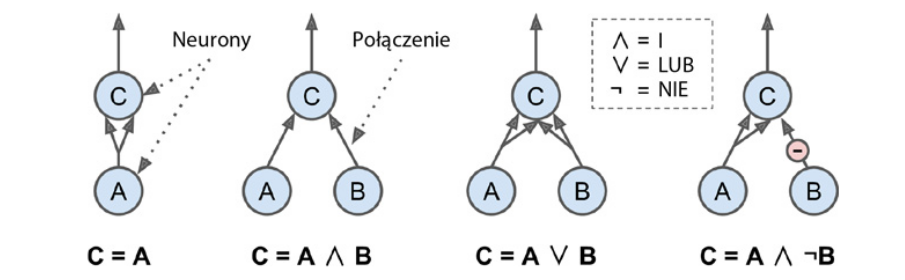
\includegraphics[width=9cm]{rys/neurony1.png}
	\caption{Przykładowe sztuczne sieci neuronowe rozwiązujące proste zadania logiczne}
	\zrodlo{\cite{geron}}
	\label{fig:neurony1}
\end{figure}

Jedną z najprostszych architektur SSN jest \textbf{perceptron}, którego podstawą jest sztuczny neuron zwany \textbf{progową jednostką logiczną} (ang. \textit{Threshold Logic Unit} - TLU) lub \textbf{liniową jednostką progową} (ang. \textit{Linear Threshold Unit} - LTU). Wartościami wejść i wyjść są liczby, a każde połączenie ma przyporządkowaną wagę. Jednostka TLU oblicza ważoną sumę sygnałów wejściowych, a następnie zostaje użyta funkcja skokowa. Schemat takiej jednostki został przedstawiony na rysunku \ref{fig:neurony2}.

\begin{figure}[!h]
	\centering
	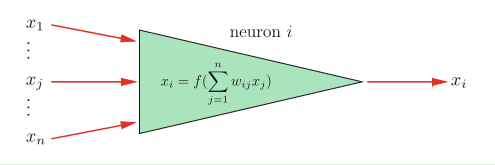
\includegraphics[width=8cm]{rys/neurony2.png}
	\caption{Struktura sztucznego neuronu, który stosuje funkcję skokową $f$ na ważonej sumie sygnałów wejściowych}
	\zrodlo{\cite{ertel}}
	\label{fig:neurony2}
\end{figure}

Często używaną funkcją skokową jest \textbf{funkcja Heaviside'a}, określona równaniem 

$$H(z)=\begin{cases}
0, & \text{ jeśli } z<0\\
1, & \text{ jeśli } z \geq 0
\end{cases}$$

Czasami stosuje się również \textbf{funkcję signum}

$$sgn(z)=\begin{cases}
-1 & \text{ jeśli } z<0\\
0, & \text{ jeśli } z=0\\
1, & \text{ jeśli } z > 0
\end{cases}$$

Perceptron jest złożony z jednej warstwy jednostek TLU, w której każdy neuron jest połączony ze wszystkimi wejściami. Tego typu warstwa jest nazywana \textbf{warstwą gęstą}. Warstwa, do której są dostarczane dane wejściowe, jest nazywana \textbf{warstwą wejściową} (ang. \textit{input layer}). Najczęściej do tej warstwy jest wstawiany również \textbf{neuron obciążeniowy} (ang. \textit{bias neuron}) $x_0=1$, który zawsze wysyła wartość 1. Na rysunku \ref{fig:perceptron1} znajduje się perceptron z dwoma neuronami wejściowymi i jednym obciążeniowym, a także z trzema neuronami w warstwie wyjściowej.

\begin{figure}[!h]
	\centering
	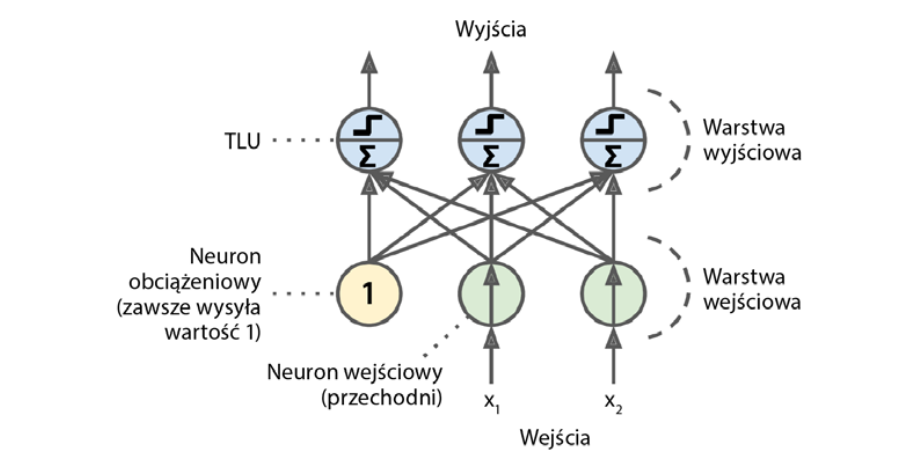
\includegraphics[width=10cm]{rys/perceptron1.png}
	\caption{Perceptron z trzema neuronami wejściowymi i trzema wyjściami}
	\zrodlo{\cite{geron}}
	\label{fig:perceptron1}
\end{figure}

Obliczanie sygnałów wyjściowych w warstwie gęstej przedstawia się wzorem
$$h_{\mathbf{W},\mathbf{b}}(\mathbf{X})=\phi(\mathbf{XW}+\mathbf{b})$$
gdzie $\mathbf{X}$ - macierz cech wejściowych, $\mathbf{W}$ - macierz wag połączeń (oprócz neuronu obciążeniowego), $\mathbf{b}$ - wektor obciążeń zawierający wagi połączeń neuronu obciążeniowego ze wszystkimi innymi neuronami, $\phi$ - tzw. \textbf{funkcja aktywacji}, w przypadku TLU jest to funkcja skokowa.

Algorytm uczący, który służy do trenowania perceptronu, jest silnie inspirowany działaniem neuronu biologicznego. Gdy biologiczny neuron często pobudza inną komórkę nerwową, to połączenia między nimi stają się silniejsze. Reguła ta jest nazywana \textbf{regułą Hebba}. Perceptrony są uczone za pomocą odmiany tej reguły, w której połączenia są wzmacniane, jeśli pomagają zmniejszyć wartość błędu. Dokładniej, w danym momencie perceptron przetwarza jeden przykład uczący i wylicza dla niego predykcję. Na każdy neuron wyjściowy odpowiadający za nieprawidłową prognozę następuje zwiększenie wag połączeń ze wszystkimi wejściami przyczyniającymi się do właściwej prognozy. Aktualizowanie wag przedstawia się następującym wzorem
$$\Delta w_{ij}=\eta (y_j-\hat{y_j})x_i$$
gdzie $w_{ij}$ - waga połączenia między $i$-tym neuronem wejściowym a $j$-tym neuronem wyjściowym, $x_i$ - $i$-ta wartość wejściowa bieżącego przykładu uczącego, $\hat{y_j}$ - wynik $j$-tego neuronu wyjściowego dla bieżącego przykładu uczącego, $y_j$ - docelowy wynik $j$-tego neuronu, $\eta$ - współczynnik uczenia.

Perceptron ma wiele wad związanych z niemożnością rozwiązania pewnych trywialnych problemów (np. zadanie klasyfikacji rozłącznej czyli XOR). Część tych ograniczeń można wyeliminować, stosując architekturę SSN złożoną z wielu warstw perceptronów, czyli \textbf{perceptron wielowarstwowy} (ang. \emph{Multi-Layer Perceptron}). Składa się on z jednej warstwy wejściowej (przechodniej), co najmniej jednej warstwy jednostek TLU - tzw. \textbf{warstwy ukryte} (ang. \emph{latent layers}) i ostatniej warstwy jednostek TLU - warstwy wyjściowej. Oprócz warstwy wejściowej każda warstwa zawiera neuron obciążający i jest w pełni połączona z następną wartswą. Sieć zawierająca wiele warstw ukrytych nazywamy \textbf{głęboką siecią neuronową} (ang. \emph{Deep Neural Network} - DNN). 

Do uczenia perceptronów wielowarstwowych wykorzystywany jest algorytm \textbf{propagacji wstecznej} (ang. \emph{backpropagation}). Propagacja wsteczna jest właściwie algorytmem gradientu prostego \cite{skansi}. Można go zapisać jako
$$w_{updated}=w_{old}-\eta \nabla E$$
gdzie $E$ jest funkcją kosztu (funkcją straty) \cite{skansi}. Proces jest powtarzany do momentu uzyskania zbieżności z rozwiązaniem, a każdy przebieg jest nazywany \textbf{epoką} (ang. \emph{epoch}).

\begin{uwaga}
	Wagi połączeń wszystkich warstw ukrytych należy koniecznie zainicjować losowo. W przeciwnym przypadku proces uczenia zakończy się niepowodzeniem. Na przykład jeśli wszystkie wagi i obciążenia zostaną zainicjowane wartością 0, to model będzie działał tak, jak gdyby składał się tylko z jednego neuronu. Przy zainicjowaniu wag losowo, symetria zostanie złamana i algorytm propagacji wstecznej będzie w stanie wytrenować zespół zróżnicowanych neuronów \cite{geron}. 
\end{uwaga}

Aby algorytm propagacji wstecznej działał prawidłowo, kluczową zmianą jest zastąpienie funkcji skokowej przez inne \textbf{funkcje aktywacji}. Zmiana ta jest konieczna, ponieważ funkcja skokowa zawiera jedynie płaskie segmenty i przez to nie pozwala korzystać z gradientu. 

Najczęściej używana jest \textbf{funkcja logistyczna (sigmoidalna)}
$$\sigma(z)=\frac{1}{1+e^{-z}}$$
Ma ona w każdym punkcie zdefiniowaną pochodną niezerową, dzięki czemu algorytm gradientu prostego może na każdym etapie uzyskać lepsze wyniki. Zbiór wartości tej funkcji wynosi od 0 do 1.

Inną popularną funkcją aktywacji jest \textbf{tangens hiperboliczny}
$$\operatorname{tanh}(z)=2\sigma(2z)-1$$
Funkcja ta jest ciągła i różniczkowalna, a jej zakres wartości wynosi $-1$ do 1. Dzięki temu zakresowi wartości wynik każdej warstwy jest wyśrodkowany wobec zera na początku uczenia, co często pomaga w szybszym uzyskaniu zbieżności.

Wśród popularnych funkcji aktywacji należy także wyróżnić  \textbf{funkcję ReLU} (ang. \emph{Rectified Linear Unit} - prostowana jednostka liniowa) o wzorze
$$ReLU(z)=max(0,z).$$
Jest ona ciągła, ale nieróżniczkowalna w punkcie 0. Jej pochodna dla $z<0$ wynosi zero. Jej atutem jest szybkość przetwarzania. Nie ma ona maksymalnej wartości wyjściowej.
W zadaniach regresji bywa wykorzystywany ,,wygładzony'' wariant funkcji ReLU, czyli funkcja \textbf{softplus}:
$$softplus(z)=log(1+exp(z))$$

Na  rysunku \ref{fig:funkcje-aktywacji} przedstawiono popularne funkcje aktywacji wraz z ich pochodnymi.

\begin{figure}[!h]
	\centering
	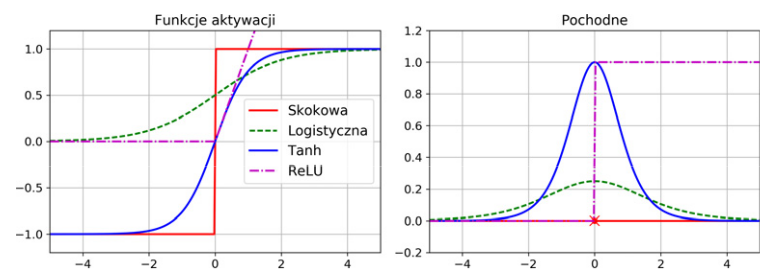
\includegraphics[width=\linewidth]{rys/funkcje_aktywacji.png}
	\caption{Przykładowe funkcje aktywacji wraz z pochodnymi}
	\zrodlo{\cite{geron}}
	\label{fig:funkcje-aktywacji}
\end{figure}

\section{Sieci splotowe}

Sieci splotowe, nazywane również \textbf{splotowymi sieciami neuronowymi} (ang. \emph{convolutional neural networks}, CNN), są rodzajem sieci neuronowych służących do przetwarzania danych o znanej topologii siatki. Przykładem takich danych są szeregi czasowe, które można uznać za jednowymiarową siatkę z próbkami w regularnych odstępach czasu, oraz dane graficzne, które można interpretować jako dwuwymiarową siatkę pikseli. Nazwa sieci splotowych pochodzi od wykorzystywanego przez te sieci działania matematycznego nazywanego \textbf{splotem} (konwolucją). Można powiedzieć, że sieci splotowe to po prostu sieci neuronowe, które w przynajmniej jednej z warstw zamiast ogólnego mnożenia macierzy wykorzystują splot \cite{goodfellow}.


\cite{geron}

Splotowe sieci neuronowe stanowią wynik badań nad korą wzrokową. Są używane głównie do rozpoznawania obrazów (od lat 80-tych XX w.).

Zagadnienia rozpoznawania obrazu:
\begin{itemize}
	\item klasyfikacja
	\item detekcja obrazów
	\item transfer stylu
\end{itemize}

Neurony biologiczne w korze wzrokowej reagują na określone wzorce w niewielkich obszarach pola wzrokowego, zwanych polami recepcyjnymi; w miarę przepływu sygnału wzrokowego przez kolejne moduły w mózgu neurony rozpoznają coraz bardziej skomplikowane wzorce wykrywane w coraz większych polach recepcyjnych.

Wiele neuronów tworzących korę wzrokową tworzą lokalne pola recepcyjne, reagujące jedynie na bodźce wzrokowe mieszczące się w określonym rejonie pola wzrokowego.

Pola recepcyjne poszczególnych neuronów mogą się na siebie nakładać.

Pola recepcyjne łącznie tworzą całe pole wzrokowe.

Pewne neurony reagują wyłącznie na obrazy składające się z linii poziomych, lub innych linii ułożonych w konkretny sposób.

Niektóre komórki nerwowe mają większe pola recepcyjne i wykrywają bardziej skomplikowane kształty.

Neurony odpowiedzialne za rozpoznawanie bardziej skomplikowanych kształtów znajdują się na wyjściu neuronów reagujących na prostsze bodźce.

\cite{geron}

Splotowe (konwolucyjne) sieci neuronowe (ang. convolutional neural networks — CNN) stanowią
wynik badań nad korą wzrokową i od lat 80. ubiegłego wieku są używane do rozpoznawania obrazów.
W ciągu kilku ostatnich lat sieci CNN zdołały osiągnąć wyniki przekraczające ludzkie możliwości
w pewnych skomplikowanych zadaniach wizualnych; stało się to możliwe dzięki wzrostowi mocy
obliczeniowej, ilości dostępnych danych uczących i opisanym w rozdziale 11. sposobom uczenia
sztucznych sieci neuronowych. Stanowią one podstawę usług wyszukiwania obrazów, samochodów
inteligentnych, zautomatyzowanych systemów klasyfikowania filmów itd. Co więcej, splotowe
sieci neuronowe nie ograniczają się wyłącznie do postrzegania obrazów: okazują się również skuteczne
w innych zadaniach, takich jak rozpoznawanie mowy (ang. voice recognition) czy przetwarzanie
języka naturalnego (ang. natural language processing — NLP).
\begin{figure}[!h]
	\centering
	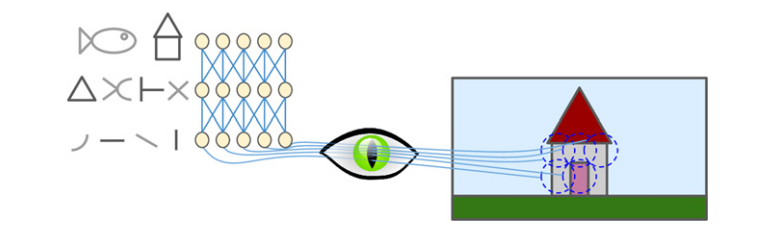
\includegraphics[width=\linewidth]{rys/kora_wzrokowa.png}
	\caption{Neurony biologiczne w korze wzrokowej reagują na określone wzorce w niewielkich obszarach
		pola wzrokowego, zwanych polami recepcyjnymi; w miarę przepływu sygnału wzrokowego przez kolejne
		moduły w mózgu neurony rozpoznają coraz bardziej skomplikowane wzorce wykrywane w coraz większych
		polach recepcyjnych}
	\zrodlo{\cite{geron}}
	\label{fig:kora-wzrokowa}
\end{figure}


Warstwy splotowe
Najistotniejszym składnikiem sieci CNN jest warstwa splotowa (konwolucyjna; ang. convolutional
layer) 6 : neurony w pierwszej warstwie splotowej nie są połączone z każdym pikselem obrazu wejścio-
wego (w przeciwieństwie do sieci opisanych w poprzednich rozdziałach), lecz wyłącznie z pikselami
znajdującymi się w ich polu recepcyjnym (rysunek 14.2). Z kolei każdy neuron w drugiej warstwie
splotowej łączy się wyłącznie z neuronami znajdującymi się w niewielkim obszarze pierwszej war-
stwy. Dzięki temu sieć może koncentrować się na ogólnych cechach w pierwszej warstwie ukrytej,
następnie łączyć je w bardziej złożone kształty w drugiej warstwie ukrytej itd. Taka hierarchiczna
struktura jest powszechnie spotykana na zdjęciach, co stanowi jedną z przyczyn tak dużej skuteczności
sieci CNN w rozpoznawaniu obrazów.
\begin{figure}[!h]
	\centering
	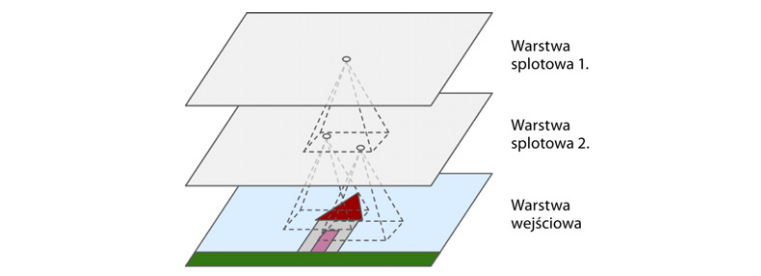
\includegraphics[width=\linewidth]{rys/warstwy_cnn.png}
	\caption{Warstwy CNN z prostokątnymi lokalnymi polami recepcyjnymi}
	\zrodlo{\cite{geron}}
	\label{fig:warstwy-cnn}
\end{figure}
Neuron znajdujący się w wierszu $i$ oraz kolumnie $j$ danej warstwy jest połączony z wyjściami neuro-
nów poprzedniej warstwy zlokalizowanymi w rzędach od $i$ do $i+f_h -1$ i kolumnach od $j$ do $j+f_w -1$,
gdzie $f_h$ i $f_w$ oznaczają, odpowiednio, wysokość i szerokość pola recepcyjnego (rysunek 14.3). W celu
uzyskania takich samych wymiarów każdej warstwy najczęściej są dodawane zera wokół wejść, co zo-
stało pokazane na rysunku 14.3. Proces ten nazywamy uzupełnianiem zerami (ang. zero padding).
\begin{figure}[!h]
	\centering
	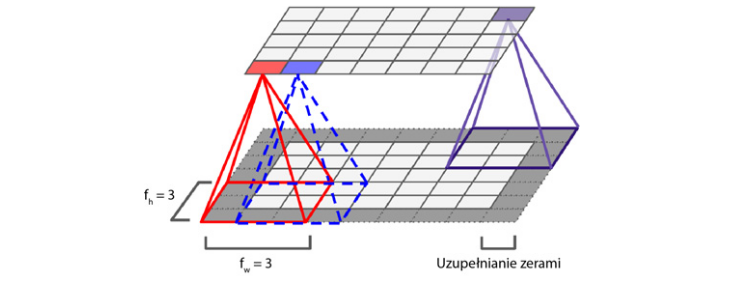
\includegraphics[width=\linewidth]{rys/zero_padding.png}
	\caption{Związek pomiędzy warstwami a uzupełnianiem zerami}
	\zrodlo{\cite{geron}}
	\label{fig:zero-padding}
\end{figure}
Możliwe jest również łączenie bardzo dużej warstwy wejściowej ze znacznie mniejszą kolejną warstwą
poprzez rozdzielanie pól recepcyjnych, tak jak zaprezentowano na rysunku 14.4. Rozwiązanie to
zmniejsza drastycznie złożoność obliczeniową modelu. Odległość pomiędzy dwoma kolejnymi polami
recepcyjnymi nosi nazwę kroku (ang. stride). Na widocznym schemacie warstwa wejściowa o wymia-
rach 5×7 (plus uzupełnianie zerami) łączy się z warstwą o rozmiarze 3×4 za pomocą pól recepcyj-
nych będących kwadratami 3×3 i kroku o wartości 2 (w omawianym przykładzie krok jest taki sam
w obydwu wymiarach, ale nie jest to wcale regułą). Neuron zlokalizowany w rzędzie $i$ oraz kolumnie $j$
górnej warstwy łączy się z wyjściami neuronów dolnej warstwy mieszczącymi się w rzędach od
$i\times s_h$ do $i\times s_h +f_h -1$ i w kolumnach od $j\times s_w$ do $j \times s_w +f_w -1$, gdzie $s_h$ i $s_w$ definiują wartości kroków od-
powiednio w kolumnach i rzędach.

Filtry
Wagi neuronu mogą być przedstawiane jako niewielki obraz o rozmiarze pola recepcyjnego. Na
przykład na rysunku 14.5 widzimy dwa możliwe zbiory wag, tak zwane filtry (lub jądra splotowe;
ang. convolution kernels). Pierwszy filtr jest symbolizowany jako czarny kwadrat z białą pionową
linią przechodzącą przez jego środek (jest to macierz o wymiarach 7×7 wypełniona zerami oprócz
środkowej kolumny, która zawiera jedynki); neurony zawierające te wagi będą ignorować wszystkie
elementy w polu recepcyjnym oprócz znajdujących się w środkowej pionowej linii (dane wejściowe
znajdujące się poza tą linią będą przemnażane przez 0). Drugi filtr wygląda podobnie; różnica
polega na tym, że środkowa linia jest ułożona poziomo. Także w tym wypadku będą brane pod uwagę
jedynie dane wejściowe znajdujące się w tej linii.
Jeśli wszystkie neurony w danej warstwie będą korzystać z tego samego filtra „pionowego” (i takiego
samego członu obciążenia), a my wczytamy do sieci obraz zaprezentowany na dole rysunku 14.5,
to uzyskamy obraz widoczny w lewym górnym rogu rysunku. Zauważ, że po zastosowaniu tego filtru
pionowe białe linie stają się wyraźniej widoczne, natomiast pozostała część obrazu zostaje rozmazana.
Na zasadzie analogii otrzymujemy obraz widoczny w prawym górnym rogu rysunku po zastosowa-
niu filtru „poziomego”; teraz z kolei białe poziome linie zostają wyostrzone, a reszta obrazu ulega
zamazaniu. Zatem warstwa wypełniona neuronami wykorzystującymi ten sam filtr daje nam mapę
cech (ang. feature map), dzięki której możemy dostrzec elementy najbardziej przypominające dany
filtr. Nie musisz oczywiście definiować filtrów własnoręcznie — sieć CNN w czasie uczenia wy-
szukuje filtry najbardziej przydatne do danego zadania i uczy się łączyć je w bardziej złożone
wzorce.


Stosy map cech
Do tej pory dla uproszczenia przedstawialiśmy każdą warstwę splotową w postaci cienkiej, dwuwymia-
rowej warstwy, ale w rzeczywistości składa się ona z kilku map cech o identycznych rozmiarach,
dlatego trójwymiarowe odwzorowanie jest bliższe rzeczywistości (rysunek 14.6). W zakresie jed-
nej mapy cech każdy neuron jest przydzielony do jednego piksela, a wszystkie tworzące ją neurony
współdzielą te same parametry (wagi i człon obciążenia). Neurony w innych mapach cech mają od-
mienne wartości parametrów. Pole recepcyjne neuronu nie ulega zmianie, ale „przebiega” przez
wszystkie mapy cech poprzednich warstw. Krótko mówiąc, warstwa splotowa równocześnie stosuje
różne filtry na wejściach, dzięki czemu jest w stanie wykrywać wiele cech w dowolnym obszarze obrazu.

Co więcej, obrazy wejściowe także składają się z kilku warstw podrzędnych, po jednej na każdy kanał
barw (ang. color channel). Standardowo występują trzy kanały barw — czerwony, zielony i niebieski
(ang. red, green, blue — RGB). Obrazy czarno-białe (w odcieniach szarości) zawierają tylko jeden
kanał, ale istnieją też takie zdjęcia, które mogą mieć ich znacznie więcej — np. fotografie satelitarne
utrwalające dodatkowe częstotliwości fal elektromagnetycznych (takie jak podczerwień).

W szczególności neuron zlokalizowany w rzędzie $i$ oraz kolumnie $j$ mapy cech $k$ w danej warstwie
splotowej $l$ jest połączony z neuronami wcześniejszej warstwy $l-1$ umieszczonymi w rzędach od $i\times s_h$
do $i\times s_h +f_h -1$ i kolumnach od $j\times s$ w do $j\times s_w +f_w -1$ we wszystkich mapach cech (warstwy $l-1$). Zwróć
uwagę, że wszystkie neurony znajdujące się w tym samym rzędzie $i$ oraz kolumnie $j$, ale w innych
mapach cech są połączone z wyjściami dokładnie tych samych neuronów poprzedniej warstwy.

\begin{figure}[!h]
	\centering
	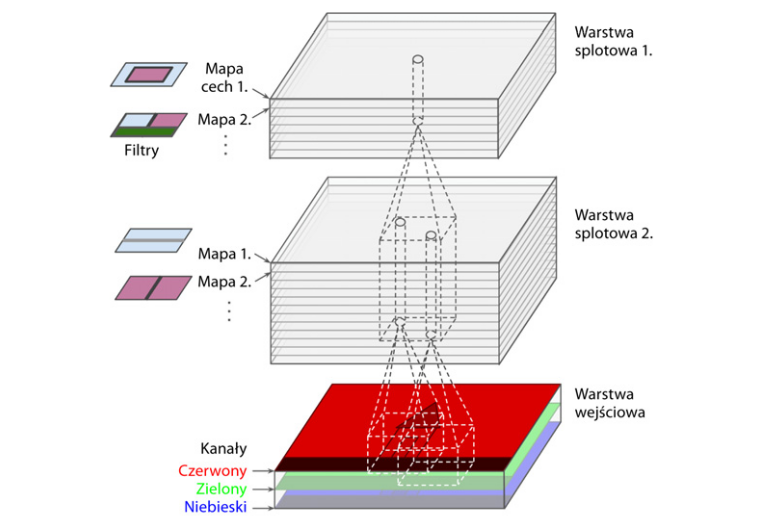
\includegraphics[width=\linewidth]{rys/warstwy_cnn_kanaly.png}
	\caption{Warstwy splotowe zawierające wiele map cech, a także zdjęcie z trzema kanałami barw}
	\zrodlo{\cite{geron}}
	\label{fig:warstwy-kanaly}
\end{figure}

Powyższy opis został podsumowany w równaniu 14.1: widoczny duży wzór matematyczny służy
do obliczania wyniku danego neuronu w warstwie splotowej. Z powodu dużej liczby indeksów
równanie to nie wygląda zbyt elegancko, ale za jego pomocą jesteśmy w stanie uzyskać sumę ważoną
wszystkich danych wejściowych wraz z członem obciążenia.
$$z_{i,j,k}=b_k\sum_{u=0}^{f_h-1}\sum_{v=0}^{f_w-1}\sum_{k'=0}^{f_{n'}-1}x_{i', j', k'} \cdot w_{u,v,k', k},\text{~~~gdzie }\begin{cases}
i'=i \times s_h+u\\
j'=j \times s_w+v
\end{cases}$$
W tym równaniu:
\begin{itemize}
	\item $z_{i,j,k}$ jest wyjściem neuronu znajdującego się w rzędzie $i$, kolumnie $j$ i mapie cech $k$ warstwy
	splotowej $l$;
	\item jak już zostało wyjaśnione, $s_h$ i $s_w$ to kroki pionowy i poziomy, $f_h$ i $f_w$ są wysokością i szerokością
	pola recepcyjnego, natomiast $f_{n'}$ oznacza liczbę map cech w poprzedniej warstwie $(l-1)$;
	\item $x_{i',j',k'}$ jest wyjściem neuronu zlokalizowanego w warstwie $l-1$, rzędzie $i'$, kolumnie $j'$, mapie
	cech $k$ (lub kanale $k'$, jeżeli poprzednia warstwa była warstwą wejściową);
	\item $b_k$ to człon obciążenia dla mapy cech $k$ (w warstwie $l$); można go interpretować jako „pokrętło
	jasności” mapy cech $k$;
	\item $w_{u,v,k',k}$ jest wagą połączenia pomiędzy dowolnym neuronem w mapie cech $k$ warstwy $l$ a jego
	wejściem mieszczącym się w wierszu $u$, kolumnie $v$ (względem pola recepcyjnego neuronu)
	a mapą cech $k'$.
\end{itemize}


Przejdźmy teraz do drugiego elementu budulcowego sieci CNN — warstwy łączącej.
Warstwa łącząca
Gdy już wiemy, jak działa warstwa splotowa, zrozumienie mechanizmu kryjącego się za warstwami
łączącymi (ang. pooling layers) nie powinno stanowić problemu. Ich celem jest podpróbkowanie
(ang. subsample; tj. zmniejszenie) obrazu wejściowego w celu zredukowania obciążenia obliczeniowego,
wykorzystania pamięci i liczby parametrów (a tym samym ograniczenia ryzyka przetrenowania).
Podobnie jak w przypadku warstw splotowych, każdy neuron stanowiący część warstwy łączącej
łączy się z wyjściami określonej liczby neuronów warstwy poprzedniej, mieszczącej się w obszarze
niewielkiego, prostokątnego pola recepcyjnego. Podobnie jak wcześniej, musimy definiować tu
rozmiar tego pola, wartość kroku, rodzaj uzupełniania zerami itd. Jednakże warstwa łącząca nie zawiera
żadnych wag; jej jedynym zadaniem jest gromadzenie danych wejściowych za pomocą jakiejś funk-
cji agregacyjnej, np. maksymalizującej lub uśredniającej. Na rysunku 14.8 widzimy najpopularniejszy
rodzaj — maksymalizującą warstwę łączącą (ang. max pooling layer). W tym przykładzie korzystamy
z jądra łączącego 9 (ang. pooling kernel) o rozmiarze 2×2, kroku o wartości 2 i z pominięciem uzupeł-
niania zerami. Zwróć uwagę, że jedynie maksymalna wartość z każdego jądra zostaje przekazana do
następnej warstwy natomiast pozostałe wartości wejściowe zostają odrzucone. Na przykład w lewym
dolnym polu recepcyjnym na rysunku 14.8 widzimy wartości wejściowe 1, 5, 3, 2, zatem tylko wartość
maksymalna (5) zostanie przekazana do następnej warstwy. Z powodu kroku równego 2 obraz wyj-
ściowy ma szerokość i wysokość o połowę mniejsze w porównaniu do obrazu wejściowego (zaokrą-
glamy tu w dół, ponieważ nie korzystamy z uzupełniania zerami).

\begin{figure}[!h]
	\centering
	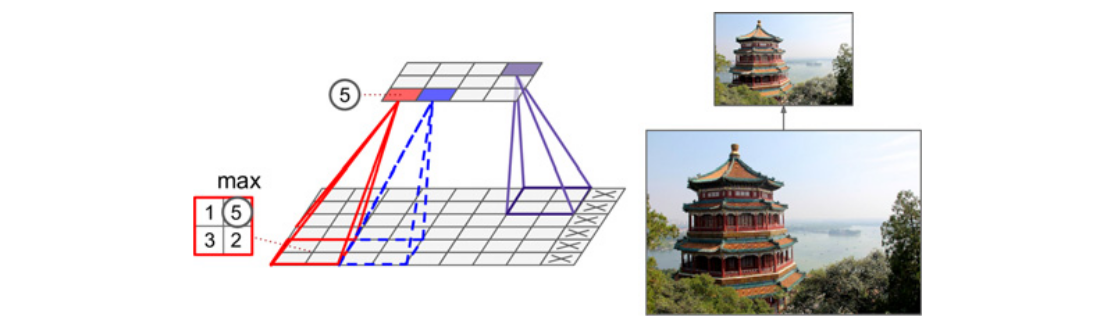
\includegraphics[width=\linewidth]{rys/max_pooling_layer.png}
	\caption{Maksymalizująca warstwa łącząca (jądro łączące: 2×2, krok: 2, brak uzupełniania zerami)}
	\zrodlo{\cite{geron}}
	\label{fig:max-pooling-layer}
\end{figure}
Oprócz ograniczania liczby obliczeń, zużycia pamięci i liczby parametrów maksymalizująca war-
stwa łącząca wprowadza także pewien stopień niezmienniczości w stosunku do drobnych prze-
sunięć, co widać na rysunku 14.9. Zakładamy tu, że piksele jasne mają mniejszą wartość od pikseli
ciemnych, trzy obrazy (A, B i C) przechodzą przez maksymalizującą warstwę łączącą o jądrze 2×2
i kroku równym 2. Obrazy B i C wyglądają tak samo jak obraz A, ale są przesunięte o, odpowied-
nio, jeden i dwa piksele w prawo. Jak widać, rezultaty wygenerowane w maksymalizującej warstwie
łączącej z obrazów A i B są identyczne. Na tym polega niezmienniczość przesunięć (ang. translation
invariance). W przypadku obrazu C wynik jest odmienny: jest on przesunięty o jeden piksel w prawo
(nadal jednak pozostaje niezmieniony w mniej więcej 75%). Poprzez wstawianie maksymalizują-
cej warstwy łączącej co kilka warstw sieci CNN możliwe jest uzyskanie ograniczonej niezmienni-
czości przesunięć w większej skali. Ponadto warstwa ta zapewnia niewielki stopień niezmienni-
czości rotacyjnej i drobną niezmienniczość skalowania. Tego typu niezmienniczość (mimo że jest
ograniczona) przydaje się wszędzie tam, gdzie prognozy nie powinny być zależne od tych szcze-
gółów, na przykład w zadaniach klasyfikacji.
\begin{figure}[!h]
	\centering
	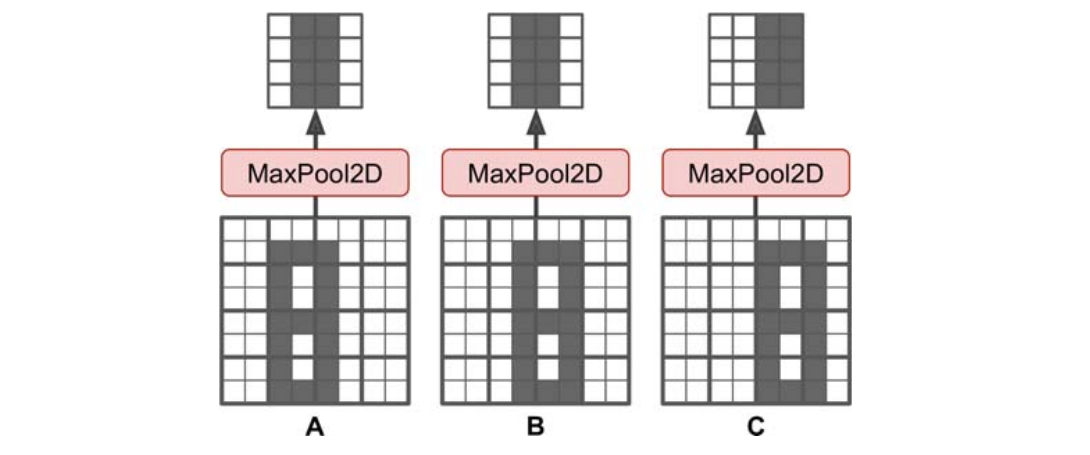
\includegraphics[width=\linewidth]{rys/niezmienniczosc_pooling.png}
	\caption{Niezmienniczość związana z drobnymi przesunięciami}
	\zrodlo{\cite{geron}}
	\label{fig:niezmienniczosc-pooling}
\end{figure}
Jednak maksymalizująca warstwa łącząca jest niepozbawiona również wad. Przede wszystkim jest
ona bardzo niszczycielska: nawet w przypadku niewielkiego jądra o rozmiarze 2×2 i kroku o wartości 2
dane wyjściowe będą dwukrotnie mniejsze w każdym kierunku (zatem obszar obrazu będzie
zmniejszony czterokrotnie), co oznacza porzucenie 75% wartości wejściowych. Z kolei w pewnych
zastosowaniach niezmienniczość jest niepożądana, dajmy na to w segmentacji semantycznej (zadaniu
klasyfikowania każdego piksela obrazu zgodnie z jego przynależnością do danego obiektu; później
wrócimy do tego zagadnienia): jest oczywiste, że jeżeli obraz wejściowy zostanie przesunięty o jeden
piksel w prawo, to wynik również powinien być przesunięty w taki sam sposób. Wówczas celem staje
się ekwiwariancja (ang. equivariance), a nie niezmienniczość: mała zmiana w sygnale wejściowym
powinna prowadzić do powiązanej z nią niewielkiej zmiany w sygnale wyjściowym.


Ostatnim rodzajem warstwy łączącej często spotykanym we współczesnych architekturach jest
globalna uśredniająca warstwa łącząca (ang. global average pooling layer). Mechanizm jej działania
jest całkiem odmienny: oblicza ona jedynie średnią każdej mapy cech (przypomina to działanie
uśredniającej warstwy łączącej, w której jądro ma takie same wymiary przestrzenne jak dane
wejściowe). Oznacza to, że generuje ona na wyjściu pojedynczą wartość na każdą mapę cech
i na każdy przykład. Jest to oczywiście rozwiązanie skrajnie destrukcyjne (większość informacji
zawartych w mapie cech zostaje utraconych), ale, jak przekonasz się w dalszej części rozdziału,
bywa przydatne na wyjściu modelu.

\subsection{Hiperparametry filtru konwolucyjnego}

\cite{illustrated}

Warstwy konwolucyjne w przeciwieństwie do zagęszczonych, nie są w pełni połączone. Oznacza to, że w pierwszej warstwie ukrytej nie są wiązane wagi wszystkich pikseli ze wszystkimi neuronami. Zamiast tego stosowanych jest kilka wymienionych niżej hiperparametrów określających liczbę wag i odchyleń związanych z daną warstwą konwolucyjną:
\begin{itemize}
	\item wielkość jądra (kernel size) - jądro (zwane również filtrem lub polem receptywnym) typowo ma wysokość i szerokość trzech pikseli. Rozmiar ten okazał się optymalny w szerokim zakresie zastosowań widzenia maszynowego w nowoczesnych sieciach konwolucyjnych. Popularna jest również wielkość 5x5 pikseli, a maksymalny stosowany rozmiar to 7x7 pikseli. Jeśli jądro jest zbyt duże w stosunku do obrazu, wtedy w polu receptywnym pojawia się zbyt wiele cech i warstwa konwolucyjna nie jest w stanie się skutecznie uczyć. Jeżeli jądro jest zbyt małe, np. ma wymiary 2x2 piksele, nie jest w stanie dopasować się do żadnej struktury, przez co jest bezużyteczne.
	
	\item długość kroku (stride length) - oznacza odległość, o jaką jądro przesuwa się po obrazie. Często stosowaną wielkością jest długość jednego piksela. Często wybieraną długością są również dwa piksele, rzadziej trzy. Dłuższe kroki nie są stosowane, ponieważ jądro może wtedy pomijać obszary obrazu potencjalnie wartościowe dla modelu. Z drugiej strony, im dłuższy krok, tym większa szybkość uczenia się modelu, ponieważ jest mniej obliczeń do wykonania. Trzeba znajdować kompromis między tymi efektami.
	
	\item dopełnienie (padding) - jest ściśle związane z długością kroku. Zapewnia poprawność obliczeń w warstwie konwolucyjnej.
	
\end{itemize}	
	
	\subsection{Warstwy redukujące}
	
	\cite{illustrated}
	
	Warstwy konwolucyjne często współpracują z innego typu warstwami, stanowiącymi fundament sieci neuronowych i widzenia maszynowego. Są to warstwy redukujące (pooling layers), których zadaniem jest zmniejszanie ogólnej liczby parametrów sieci, redukowanie złożoności, przyspieszanie obliczeń i zapobieganie nadmiernemu dopasowaniu modelu.
	
	Warstwa konwolucyjna może zawierać dowolną liczbę jąder, z których każde generuje mapę aktywacji. Zatem wyjście warstwy konwolucyjnej jest trójwymiarowa tablica aktywacji, której głębokość jest równa liczbie filtrów. Warstwa redukująca zmniejsza przestrzenny wymiar mapy aktywacji, pozostawiając jej głębokość bez zmian.
	
	Z warstwą redukującą, podobnie jak z konwolucyjną, jest związany filtr i długość kroku. Filtr przesuwa się nad danymi wejściowymi, tak jak w warstwie konwolucyjnej, i w każdej zajmowanej pozycji przeprowadza operację redukcji danych. Najczęściej jest to wybieranie największej wartości, dlatego taka warstwa jest również określana mianem maksymalnie redukującej (max-pooling layer). Z całego pola receptywnego jest wybierana największa wartość (maksymalna aktywacja), a pozostałe wartości są odrzucane. Filtr w warstwie redukującej ma zazwyczaj wymiary 2x2 piksele, a krok ma długość dwóch pikseli. W takim wypadku filtr w każdej pozycji przetwarza cztery wartości aktywacji, wybiera największą i w efekcie czterokrotnie redukuje liczbę aktywacji. Ponieważ operacja redukcji jest wykonywana niezależnie w każdym wycinku trójwymiarowej tablicy, mapa aktywacji o wymiarach 28x28 elementów i głębokości 16 wycinków jest redukowana do tablicy 14x14 elementów. Zachowywana jest jednak jej pełna głębokość 16 wycinków.
	
	\begin{figure}[!h]
		\centering
		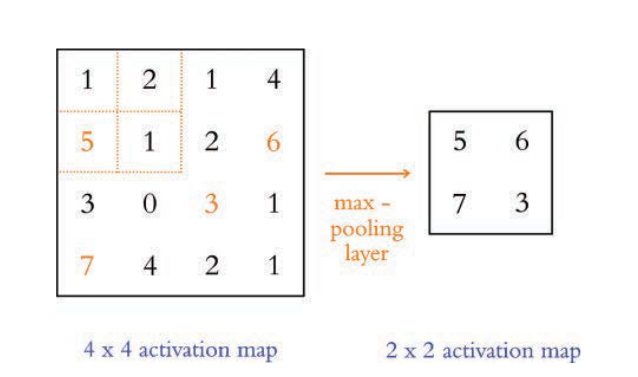
\includegraphics[width=\linewidth]{rys/max-polling.png}
		\caption{Max polling}
		\zrodlo{\cite{illustrated}}
		\label{fig:max-polling}
	\end{figure}
	
\section{Czym jest autoenkoder}

	\textbf{Autoenkoder} (czasem także nazywany autokoderem, z ang. \textit{autoencoder}, \textit{auto-encoder}) jest specjalnym typem sieci neuronowej, która jest przeznaczona głównie do kodowania danych wejściowych do skompresowanej i znaczącej reprezentacji, a następnie dekodowania ich z powrotem w taki sposób, aby zrekonstruowane dane były jak najbardziej podobne do oryginalnych \cite{bank}. Autoenkodery uczą się gęstych reprezentacji danych, tzw. reprezentacji ukrytych (ang. \emph{latent representations}) lub kodowań (ang. \emph{codings}) bez jakiejkolwiek formy nadzorowania (tzn. zbiór danych nie zawiera etykiet). Wyjściowe kodowania zazwyczaj mają mniejszą wymiarowość od danych wejściowych, dzięki czemu autoenkodery mogą z powodzeniem służyć do redukcji wymiarowości. Mają też zastosowanie w \textbf{modelach generatywnych} (ang. \emph{generative models}), które potrafią losowo generować nowe dane przypominające zbiór uczący. Jeszcze lepszej jakości dane można uzyskać przy użyciu \textbf{generatywnych sieci przeciwstawnych}, czyli GAN (ang. \textit{Generative Adversial Networks}). Sieci GAN są często stosowane w zadaniach zwiększania rozdzielczości obrazu, koloryzowania, rozbudowanego edytowania zdjęć, przekształcania prostych szkiców w realistyczne obrazy, dogenerowywania danych służących do uczenia innych modeli, generowania innych typów danych np. tekstowych, dźwiękowych, itd. \cite{geron}.


(Chapter 14 Autoencoders \cite{goodfellow})

An autoencoder is a neural network that is trained to attempt to copy its input
to its output. Internally, it has a hidden layer h that describes a code used to
represent the input. The network may be viewed as consisting of two parts: an
encoder function h = f (x) and a decoder that produces a reconstruction r = g(h).
This architecture is presented in figure 14.1 . If an autoencoder succeeds in simply
learning to set g(f (x)) = x everywhere, then it is not especially useful. Instead,
autoencoders are designed to be unable to learn to copy perfectly. Usually they are
restricted in ways that allow them to copy only approximately, and to copy only
input that resembles the training data. Because the model is forced to prioritize
which aspects of the input should be copied, it often learns useful properties of the
data.

Autoenkoder to sieć neuronowa szkolona po to, aby próbować kopiować swoje wejście do wyjścia. Wewnątrz zawiera ukrytą warstwę $h$, która opisuje kod używany do reprezentowania wejścia. Sieć można postrzegać jako składającą się z dwóch części: kodującej funkcji $h(x)$ i dekodera, który tworzy rekonstrukcję $r=g(h)$.

\begin{figure}[!h]
	\centering
	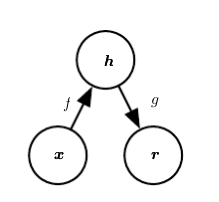
\includegraphics[width=6cm]{rys/autoencoder_structure.png}
	\caption{The general structure of an autoencoder, mapping an input x to an output
		(called reconstruction) r through an internal representation or code h. The autoencoder
		has two components: the encoder f (mapping x to h) and the decoder g (mapping h
		to r ).}
	\zrodlo{\cite{goodfellow}}
	\label{fig:autoencoder_structue}
\end{figure}

Jeśli autoenkoderowi uda się po prostu nauczyć ustawiać wszędzie $g(f(x))=x$, to wtedy nie jest zbytnio przydatny. Dlatego autoenkodery projektuje się tak, aby nie potrafiły doskonale kopiować. Zwykle nakłada się ograniczenia, aby mogły kopiować jedynie w przybliżeniu i jedynie wejście, które przypomina dane treningowe. Ponieważ model musi ustanawiać priorytety, aby ustalać, jakie aspekty wejścia powinny być kopiowane, często poznaje przydatne właściwości danych.

We współczesnych zastosowaniach oprócz deterministycznych funkcji do stochastycznego odwzorowania $p_{encoder}(h|x)$ i $p_{decoder}(x|h)$ stosuje się uogólnioną koncepcję kodera i dekodera.

Tradycyjnie autoenkodery były używane do redukcji wymiarów lub poznawania cech. Ostatnio teoretyczne powiązania z modelami zmiennych utajonych sprawiły, że autoenkodery znalazły się na pierwszym planie w modelowaniu generatywnym.

Autoenkodery można wyobrazić sobie jako specjalny przypadek sieci jednokierunkowych i można je szkolić, używając wszystkich tych samych technik, zwykle minipakietowego spadku gradientu po gradientach obliczonych przez propagację wstecz.

W przeciwieństwie to ogólnych sieci jednokierunkowych, autoenkodery można szkolić za pomocą recyrkulacji, czyli algorytmu uczącego się na bazie porównywania aktywacji sieci na oryginalnym wejściu z aktywacjami na zrekonstruowanym wejściu. 

\section{Rodzaje autoenkoderów}

Rodzaje autoenkoderów:

- niedopełniony (undercomplete)

 - regularyzowany (regularized, overcomplete)

- stosowy (stacked) lub inaczej głęboki (deep)

- splotowy (convolutional)

- rekurencyjny (recurrent)

- odszumiający (stacked denoising)

- rzadki (sparse)

- wariancyjny (variational)



\subsection{Autoenkodery niedopełnione}

\cite{goodfellow}

Copying the input to the output may sound useless, but we are typically not
interested in the output of the decoder. Instead, we hope that training the
autoencoder to perform the input copying task will result in h taking on useful
properties.
One way to obtain useful features from the autoencoder is to constrain h to
have a smaller dimension than x. An autoencoder whose code dimension is less
than the input dimension is called undercomplete. Learning an undercomplete
representation forces the autoencoder to capture the most salient features of the
training data.

The learning process is described simply as minimizing a loss function
$$L(x, g(f(x)))$$
where L is a loss function penalizing g(f(x)) for being dissimilar from x, such as
the mean squared error.
When the decoder is linear and L is the mean squared error, an undercomplete
autoencoder learns to span the same subspace as PCA.


Kopiowanie wejścia do wyjścia może wydawać się bezużyteczne, ale wyjście dekodera nas nie interesuje. Mamy za to nadzieję, że skutkiem przeszkolenia autoenkodera do kopiowania będzie kod h, mający przydatne właściwości.

Jednym ze sposobów, aby uzyskać przydatne cechy z autoenkodera, jest ograniczenie $h$ do mniejszego wymiaru niż $x$. Autoenkoder, w którym wymiar kodu jest mniejszy niż wymiar wejściowy, jest nazywany niekompletnym (niedopełnionym).

Poznawanie niekompletnych reprezentacji zmusza autoenkoder do przechwycenia najistotniejszych cech danych szkoleniowych.

Proces poznawania jest opisywany po prostu jako minimalizowanie funkcji straty
$$L(x, g(f(x)))$$
gdzie $L$ jest funkcją straty karzącą $g(f(x))$ za niepodobieństwo do $x$ jak np. błąd średniokwadratowy.

Gdy dekoder jest liniowy, a $L$ to błąd średniokwadratowy, niekompletny autoenkoder uczy się obejmować tą samą podprzestrzeń co PCA. W tym przypadku poznanie zasadniczej podprzestrzeni danych szkoleniowych przez szkolony do kopiowania autoenkoder jest efektem ubocznym. Autoenkodery z nieliniowymi funkcjami kodowania $f$ i nieliniowymi funkcjami dekodowania $g$ mogą więc poznawać potężniejsze, nieliniowe uogólnienie PCA. Niestety, jeśli koder i dekoder będą mieć zbyt dużą pojemność, autoenkoder może nauczyć się wykonywać kopiowanie bez wyodrębniania pożytecznych informacji o rozkładzie danych. Teoretycznie można sobie wyobrazić, ze autoenkoder z jednowymiarowym kodem, ale bardzo potężnym nieliniowym koderem, może nauczyć się reprezentować każdy przykład szkoleniowy $x^{(i)}$ za pomocą kodu $i$. Dekoder mógłby nauczyć się odwzorowywać te całkowitoliczbowe indeksy z powrotem na wartości konkretnych przykładów szkoleniowych. Ten konkretny przykład nie występuje w praktyce, ale pokazuje wyraźnie, że autoenkoder przeszkolony do wykonywania kopiowania może zawieść, jeśli chodzi o poznanie czegoś przydatnego na temat zbioru danych, jeśli pozwoli się, aby miał za dużą pojemność.

\subsection{Autoenkodery z regularyzacją}

\cite{goodfellow}

W przypadku, gdy wymiar wyjścia jest większy (autoenkodery nadkompletne) lub równy niż wymiar wejścia, nawet liniowy koder i dekoder mogą nauczyć się kopiować wejście do wyjścia bez uczenia się niczego przydatnego na temat rozkładu danych.

Ideałem byłaby możliwość udanego szkolenia dowolnej architektury autoenkodera przy wyborze wymiaru kodu oraz pojemności kodera i dekodera na podstawie złożoności rozkładu modelowanego. Można to zrobić, stosując regularyzację. Zamiast ograniczać pojemność modelu przez zachowywanie płytkości kodera i dekodera oraz małego rozmiaru kodu, autoenkodery z regularyzacją używają funkcji straty, dzięki której model może posiadać inne właściwości oprócz możliwości kopiowania swojego wejścia do wyjścia. Do tych właściwości należą:

\begin{itemize}
	\item  rzadkość reprezentacji
	\item mały rozmiar pochodnej reprezentacji
	\item odporność na szum lub brakujące dane wejściowe
\end{itemize}

Autoenkoder z regularyzacją może być nieliniowy i nadkompletny, a mimo to nauczyć się czegoś wartościowego o rozkładzie danych, nawet jeśli pojemność modelu jest na tyle duża, aby poznać trywialną funkcję tożsamościową.

\subsubsection{Rzadkie autoenkodery}

To autoenkoder, którego kryterium szkolenia obejmuje karę rzadkości $\Omega(h)$ na warstwie kodu $h$ oprócz błędu rekonstrukcji
$$L(x, g(f(x)))+\Omega(h)$$
gdzie $g(h)$ to wyjście dekodera, a zwykle mamy $h=f(x)$, czyli wyjście kodera.

Rzadkie autoenkodery są zwykle używane do tego, aby uczyć się cech do innego zadania, takiego jak klasyfikacja. Autoenkoder, który dzięki regularyzacji jest rzadki, musi reagować na unikatowe statystyczne cechy zbioru danych, na którym został wyszkolony, a nie tylko działać jak funkcja tożsamościowa.

\subsubsection{Autoenkodery z odszumianiem}
Zamiast dodawać karę $\Omega$ do funkcji kosztów, możemy uzyskać autoenkoder, który uczy się czegoś przydatnego, zmieniając składnik błędu rekonstrukcji w funkcji kosztów. Tradycyjne autoenkodery minimalizują jakąś funkcję
$$L(x, g(f(x)))$$
gdzie $L$ to funkcja straty karząca $g(f(x))$ za niepodobieństwo do $x$, jak np. norma $L^2$ ich różnicy. Sprzyja to temu, aby $g \circ f$  uczyła się być jedynie funkcją tożsamościową, jeśli ma do tego odpowiednią pojemność.

Autoenkoder z odszumianiem zamiast tego minimalizuje
$$L(x, g(f(\tilde{x})))$$
gdzie $\tilde{x}$ to kopia $x$, która została zniekształcona przez jakiegoś rodzaju postać szumu. Autoenkodery mają tym samym za zadanie odwrócić to zniekształcenie, a nie po prostu przekopiować swoje wejście.

\subsubsection{Regularyzacja poprzez karanie pochodnych}

kolejną strategią regularyzacji autoenkodera jest użycie kary $\Omega$ tak, jak w rzadkich autoenkoderach
$$L(x, g(f(x)))+\Omega(h,x)$$
ale z inną postacią $\Omega$:
$$\Omega(h, x)=\lambda \sum_i ||\nabla_x h_i ||^2$$
Zmusza to model do poznania funkcji, która nie zmienia się za bardzo przy niewielkich zmianach $x$. Ponieważ kara ta jest stosowana tylko w przykładach szkoleniowych, zmusza autoenkoder do poznawania cech, które przechwytują informacje o rozkładzie szkoleniowym.

Autoenkoder z taką regularyzacją jest nazywany kurczliwym.
\subsection{Autoenkodery stosowe}

(kopiowane z Gerona:)

Autokodery, podobnie jak w przypadku innych rodzajów sieci neuronowych, również mogą mieć
wiele warstw ukrytych. W takiej sytuacji są one nazywane autokoderami stosowymi (ang. stacked
autoencoders) lub głębokimi (ang. deep autoencoders). Kolejne warstwy ukryte pozwalają autokode-
rowi uczyć się bardziej skomplikowanych kodowań. Jednak musimy uważać, aby nie stworzyć
zbyt potężnego modelu. Wyobraź sobie tak wydajny autokoder, że nauczyłby się rzutować każdy
przykład wejściowy do postaci dowolnej pojedynczej liczby (a dekoder uczyłby się odwrotnego rzuto-
wania). Oczywiście taki autokoder potrafiłby doskonale rekonstruować dane uczące, ale w trakcie
tego procesu nie nauczy się żadnej przydatnej reprezentacji danych (i raczej nie będzie w stanie dobrze
generalizować przewidywań na nowe próbki).
Architektura autokodera stosowego najczęściej jest symetryczna względem centralnej warstwy ukrytej
(kodowania). Najprościej mówiąc, przypomina ona kanapkę. Na przykład autokoder klasyfikujący
obrazy MNIST (zbiór ten został opisany w rozdziale 3.) może zawierać 784 wejścia, po których nastę-
puje stuneuronowa warstwa ukryta, następnie środkowa warstwa ukryta zawierająca 30 jednostek,
a po niej kolejna stuneuronowa warstwa ukryta przechodząca w warstwę wyjściową mającą 784 wyj-
ścia.


\begin{figure}[!h]
	\centering
	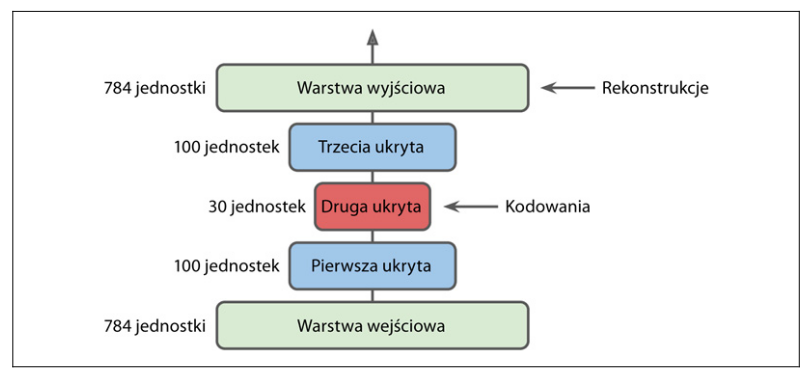
\includegraphics[width=\linewidth]{rys/autoenkoder_stosowy.png}
	\caption{Stosowy}
	\zrodlo{\cite{geron}}
	\label{fig:autoenkoder-stosowy}
\end{figure}


\subsection{Autoenkoder splotowy}

\cite{geron}

Koderem jest tradycyjna sieć splotowa składająca się z warstw splotowych i łączących. Zazwyczaj zmniejsza ona wymiarowość danych wejściowych (wysokość i szerokość
obrazu), a jednocześnie zwiększa ich głębokość (liczbę map cech). Dekoder musi przeprowadzać
odwrotną operację (zwiększyć rozdzielczość obrazu i zredukować głębokość do pierwotnej liczby
wymiarów), dlatego możemy w tym celu wykorzystać transponowane warstwy splotowe (ewentualnie możesz łączyć warstwy ekspansji z warstwami splotowymi).


\subsection{Autoenkoder rekurencyjny}

\cite{geron}

Jeżeli chcesz tworzyć autokodery przeznaczone do przetwarzania sekwencji, takich jak szeregi czasowe
czy teksty (np. nienadzorowanego uczenia wstępnego lub redukowania wymiarowości), to reku-
rencyjne sieci neuronowe (zob. rozdział 15.) mogą nadawać się do tego zadania lepiej niż sieci gęste.
Budowanie autokodera rekurencyjnego (ang. recurrent autoencoder) jest proste: koder stanowi
zazwyczaj sieć sekwencyjno-wektorową, która kompresuje sekwencję wejściową do postaci poje-
dynczego wektora. Dekoder to sieć wektorowo-sekwencyjna przeprowadzająca odwrotną operację

\begin{verbatim}
recurrent_encoder = keras.models.Sequential([
keras.layers.LSTM(100, return_sequences=True, input_shape=[None, 28]),
keras.layers.LSTM(30)
])
recurrent_decoder = keras.models.Sequential([
keras.layers.RepeatVector(28, input_shape=[30]),
keras.layers.LSTM(100, return_sequences=True),
keras.layers.TimeDistributed(keras.layers.Dense(28, activation="sigmoid"))
])
recurrent_ae = keras.models.Sequential([recurrent_encoder, recurrent_decoder])
\end{verbatim}

Taki autokoder rekurencyjny może przetwarzać sekwencje o dowolnej długości, które w każdym
takcie zawierają 28 wymiarów. Jest to dla nas dogodne, ponieważ oznacza, że możemy traktować
obrazy z zestawu Fashion MNIST tak, jakby każdy obraz stanowił sekwencję rzędów: w każdym
takcie sieć rekurencyjna będzie przetwarzać pojedynczy, 28-elementowy rząd pikseli. Oczywiście
autokoder rekurencyjny może być stosowany wobec dowolnego rodzaju sekwencji. Zwróć uwagę,że jeśli jako pierwszą warstwę dekodera wstawimy RepeatVector , to musimy sprawić, żeby w każdym
takcie do dekodera był dostarczany wektor wejściowy.


Do tej pory zmuszaliśmy autokoder do rozpoznawania interesujących cech, ograniczając rozmiar
warstwy kodowania, przez co był on niedopełniony. W rzeczywistości istnieje wiele rodzajów
ograniczeń, które możemy wykorzystać, w tym również umożliwiające stosowanie warstwy kodowa-
nia o takim samym rozmiarze jak wejściowa, a nawet jeszcze większej, co pozwala uzyskać autokoder
przepełniony (ang. overcomplete autoencoder). Sprawdźmy teraz te inne rozwiązania.

\subsection{Autoenkodey odszumiające}

\cite{geron}

Kolejną metodą zmuszania autokodera do poznawania przydatnych cech jest dodawanie szumu
do danych wejściowych i uczenie go odzyskiwania pierwotnych, niezaszumionych informacji. Pierw-
sze koncepcje wykorzystania autokoderów do odszumiania danych pojawiły się już w latach 80. ubie-
głego wieku (m.in. pomysł ten został wspomniany w pracy magisterskiej Yanna LeCuna w 1987 roku).
Pascal Vincent i in. udowodnili w publikacji z 2008 roku (https://www.iro.umontreal.ca/~vincentp/
Publications/denoising\_autoencoders\_tr1316.pdf) 5 , że autokodery mogą być również używane do
wydobywania cech. Z kolei ten sam autor i in. w artykule z 2010 roku (http://jmlr.csail.mit.edu/
papers/v11/vincent10a) 6 zaprezentowali odszumiające autokodery stosowe (ang. stacked denoising
autoencoders).
Zaszumienie może być standardowym szumem gaussowskim dodawanym do danych wejściowych lub
może przybrać postać losowo wyłączanych wejść za pomocą metody porzucania (zob. rozdział 11.).
Obydwa rozwiązania zostały pokazane na rysunku 17.8.
Implementacja nie stanowi wyzwania: jest to standardowy autokoder stosowy zawierający dodatkową
warstwę Dropout , przez którą przechodzą dane wejściowe (możesz zastąpić ją warstwą GaussianNoise ).
Jak pamiętamy, warstwa Dropout jest aktywna jedynie w fazie uczenia (podobnie jak warstwa
GaussianNoise ):
\begin{verbatim}
dropout_encoder = keras.models.Sequential([
keras.layers.Flatten(input_shape=[28, 28]),
keras.layers.Dropout(0.5),
keras.layers.Dense(100, activation="selu"),
keras.layers.Dense(30, activation="selu")
])
dropout_decoder = keras.models.Sequential([
keras.layers.Dense(100, activation="selu", input_shape=[30]),
keras.layers.Dense(28 * 28, activation="sigmoid"),
keras.layers.Reshape([28, 28])
])
dropout_ae = keras.models.Sequential([dropout_encoder, dropout_decoder])
\end{verbatim}


\begin{figure}[!h]
	\centering
	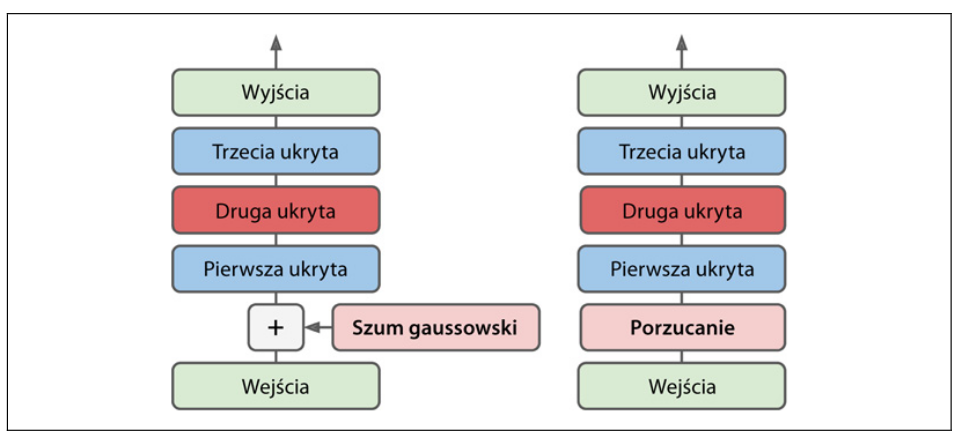
\includegraphics[width=\linewidth]{rys/autoenkoder_odszumiajacy.png}
	\caption{Autokodery odszumiające: wykorzystujące szum gaussowski (po lewej) lub metodę porzucania
		(po prawej)}
	\zrodlo{\cite{geron}}
	\label{fig:autoenkoder-odszumiajacy}
\end{figure}


Rysunek 17.9 przedstawia kilka zaszumionych obrazów (połowa pikseli została „wyłączona”), a także
ich rekonstrukcje uzyskane za pomocą autokodera odszumiającego (bazującego na warstwie po-
rzucania). Zwróć uwagę, że autokoder w istocie „zgaduje” szczegóły niewystępujące w obrazach wej-
ściowych, na przykład górną część białej sukienki (czwarty obraz w dolnym rzędzie). Jak widać,
autokodery odszumiające służą nie tylko do wizualizowania danych lub nienadzorowanego uczenia
wstępnego, lecz również w dość prosty i skuteczny sposób mogą usuwać szum z obrazów.

\begin{figure}[!h]
	\centering
	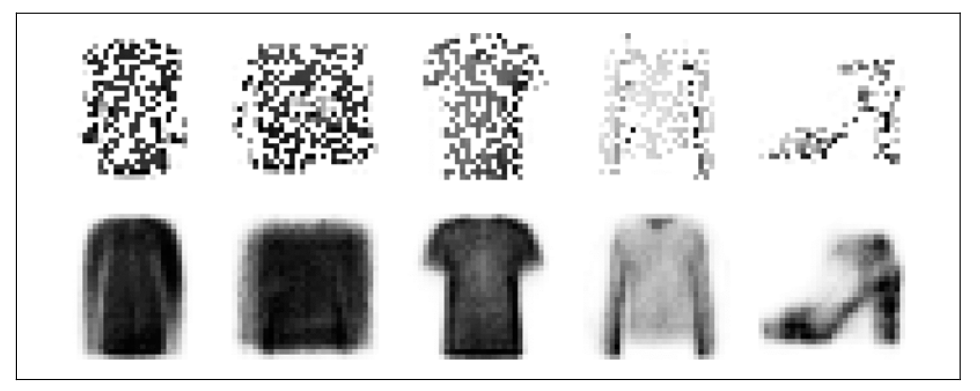
\includegraphics[width=\linewidth]{rys/denoising.png}
	\caption{Zaszumione obrazy (na górze) i ich rekonstrukcje (na dole)}
	\zrodlo{\cite{geron}}
	\label{fig:autoenkoder-denoising}
\end{figure}

\subsection{Autoenkodery rzadkie}

\cite{geron}

Innym ograniczeniem prowadzącym do skutecznego wydobywania cech jest rzadkość (ang. sparsity):
przez dodanie odpowiedniego członu do funkcji kosztu autokoder zostaje zmuszony do zmniejszenia
liczby aktywnych neuronów w warstwie kodowania. Możemy sprawić na przykład, żeby w warstwie
kodującej występowało tylko 5\% znacząco aktywnych neuronów. W ten sposób wymuszamy na auto-
koderze reprezentowanie każdego wejścia jako kombinacji niewielkiej liczby pobudzeń. Dzięki temu
każdy neuron warstwy kodowania zazwyczaj uczy się wykrywać jakąś przydatną cechę (gdybyśmy
wypowiadali w ciągu miesiąca tylko kilka słów, prawdopodobnie chcielibyśmy przekazywać za ich
pomocą wartościowe informacje).
Prostym rozwiązaniem okazuje się wprowadzenie sigmoidalnej funkcji aktywacji w warstwie kodowa-
nia (co ogranicza wartości kodowań do zakresu od 0 do 1), wprowadzenie dużej warstwy kodowania
(np. składającej się z 300 jednostek) i dodanie regularyzacji l 1 do pobudzeń warstwy kodowania
(w dekoderze nie wprowadzamy żadnych zmian):
\begin{verbatim}
sparse_l1_encoder = keras.models.Sequential([
keras.layers.Flatten(input_shape=[28, 28]),
keras.layers.Dense(100, activation="selu"),
keras.layers.Dense(300, activation="sigmoid"),
keras.layers.ActivityRegularization(l1=1e-3)
])
sparse_l1_decoder = keras.models.Sequential([
keras.layers.Dense(100, activation="selu", input_shape=[300]),
keras.layers.Dense(28 * 28, activation="sigmoid"),
keras.layers.Reshape([28, 28])
])
sparse_l1_ae = keras.models.Sequential([sparse_l1_encoder,
sparse_l1_decoder])
\end{verbatim}

Taka warstwa ActivityRegularization zwraca jedynie swoje dane wejściowe, ale jako skutek uboczny
dodaje funkcję straty uczenia równą sumie wartości bezwzględnych tychże sygnałów wejściowych
(warstwa ta jest aktywna wyłącznie w fazie uczenia). Ewentualnie możesz usunąć warstwę Activity
Regularization i wyznaczyć atrybut activity\_regularizer= keras.regularizers.l1(1e-3) w war-
stwie poprzedzającej. Kara ta będzie zmuszała sieć neuronową do tworzenia kodowań o wartościach
bliskich 0, ale jednocześnie model będzie również karany za niewłaściwe rekonstruowanie danych
wejściowych, więc będzie musiał wyznaczać co najmniej kilka wartości niezerowych. Norma l 1
sprawia, że sieć będzie przechowywała najważniejsze kodowania i eliminowała nieprzydatne z per-
spektywy obrazu wejściowego (w przeciwieństwie do normy l 2 , która jedynie redukowałaby wszystkie
kodowania).
Innym rozwiązaniem, często dającym lepsze rezultaty, jest pomiar rzeczywistej rzadkości warstwy ko-
dowania w każdym przebiegu uczenia i karanie modelu w sytuacji, gdy zmierzona rzadkość różni
się od rzadkości docelowej. Robimy to, obliczając średnią aktywację każdego neuronu w tej war-
stwie dla całej grupy próbek uczących. Rozmiar tej grupy nie może być zbyt mały, gdyż wyliczona
wartość średniej nie będzie wtedy dokładna.
Po uzyskaniu średniej wartości aktywacji każdego neuronu chcemy nałożyć karę na zbyt aktywne
neurony poprzez dodanie funkcji straty rzadkości (ang. sparsity loss) do funkcji kosztu. Przykładowo
jeśli zmierzymy średnią wartość aktywacji neuronu rzędu 0,3, ale aktywność docelowa powinna wyno-
sić 0,1, musimy zmniejszyć jego aktywność. Jednym ze sposobów jest dodanie kwadratu błędu
(0,3-0,1) 2 do funkcji kosztu, w praktyce jednak lepszym rozwiązaniem okazuje się wprowadzenie dy-
wergencji Kullbacka-Leiblera (zob. rozdział 4.), której gradienty są znacznie większe niż w błędzie
średniokwadratowym (rysunek 17.10).
\begin{figure}[!h]
	\centering
	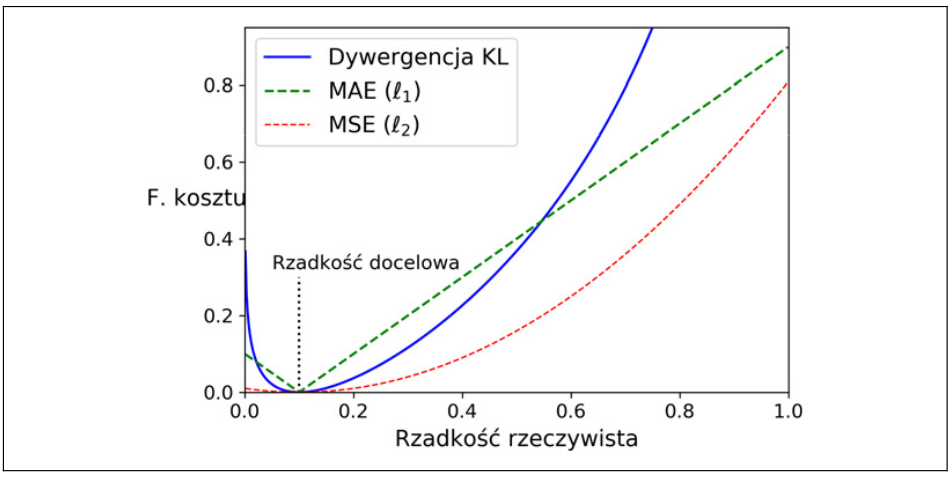
\includegraphics[width=\linewidth]{rys/funkcja_straty_rzadkosci.png}
	\caption{Funkcje straty rzadkości}
	\zrodlo{\cite{geron}}
	\label{fig:funkcja-straty-rzadkosci}
\end{figure}

Mając dwa dyskretne rozkłady prawdopodobieństwa P i Q, możemy obliczyć rozbieżność pomiędzy nimi $D_{KL}(P||Q)$ za pomocą równania 17.1. (dywergencja Kullbacka-Leiblera)

$$D_{KL}(P||Q)=\sum_i P(i)\log \frac{P(i)}{Q(i)}$$

W naszym przypadku chcemy zmierzyć rozbieżność pomiędzy docelowym prawdopodobieństwem p
aktywacji neuronu w warstwie kodowania a rzeczywistym prawdopodobieństwem q (tzn. średnią
aktywacją dla grupy przykładów uczących). Zatem dywergencja KL ulega uproszczeniu do postaci
widocznej w równaniu 17.2. (Dywergencja KL pomiędzy docelową rzadkością p a rzeczywistą rzadkością q)

$$D_{KL}(p||q)=p\log \frac{p}{q}+(1-p)\log \frac{1-p}{1-q}$$

Po obliczeniu funkcji straty rzadkości dla każdego neuronu w warstwie kodowania wystarczy je zsu-
mować i dodać wynik do funkcji kosztu. W celu regulowania względnej istotności funkcji straty
rzadkości i funkcji straty rekonstrukcji możemy pomnożyć tę pierwszą przez hiperparametr wagi
rzadkości. Jeżeli wartość wagi będzie za duża, model pozostanie blisko rzadkości docelowej, ale
jednocześnie może nie być w stanie prawidłowo rekonstruować danych wejściowych, przez co okaże się bezużyteczny. Z kolei przy zbyt małej wartości wagi rzadkości model będzie ignorował cel rzadkości
i nie nauczy się rozpoznawać przydatnych cech.

\section{Zastosowania autoenkoderów}

\url{https://towardsdatascience.com/6-applications-of-auto-encoders-every-data-scientist-should-know-dc703cbc892b}

Autoenkodery są popularnym rodzajem nienadzorowanej sztucznej sieci neuronowej, która na wejściu korzysta z nieoznakowanych danych i uczy się efektywnego kodowania struktury tych danych, które może być użyte w kontekście innych zadań. Autoenkodery aproksymują funkcję, która odwzorowuje dane z pełnej przestrzeni wejściowej na współrzędne niższego wymiaru, i dalej aproksymuje do tego samego wymiaru przestrzeni wejściowej z minimalną stratą.

W zadaniach klasyfikacji lub regresji auto-enkodery mogą być wykorzystywane do wyodrębniania cech z surowych danych w celu zwiększenia odporności modelu. Istnieje wiele innych zastosowań sieci auto-enkoderów, które można wykorzystać w innym kontekście. W tym artykule omówimy 7 takich zastosowań auto-enkodera:

1) Dimensionality Reduction (zmniejszenie wymiarowości)

2) Feature Extraction (wyodrębnianie cech)

3) Image Denoising (odszumianie obrazu)

4) Image Compression (kompresja obrazu)

5) Image Search (wyszukiwanie obrazu)

6) Anomaly Detection (wykrywanie anomalii)

7) Missing Value Imputation (uzupełnianie brakujących danych)

\subsection{Zmniejszenie wymiarowości}

(źródło jak wyżej, ale również tu: \url{https://towardsdatascience.com/autoencoders-in-practice-dimensionality-reduction-and-image-denoising-ed9b9201e7e1})

Autoenkodery trenują sieć w celu wyjaśnienia naturalnej struktury danych w efektywnej reprezentacji niskowymiarowej. Osiąga się to poprzez zastosowanie strategii dekodowania i kodowania w celu zminimalizowania błędu rekonstrukcji.

\begin{figure}[!h]
	\centering
	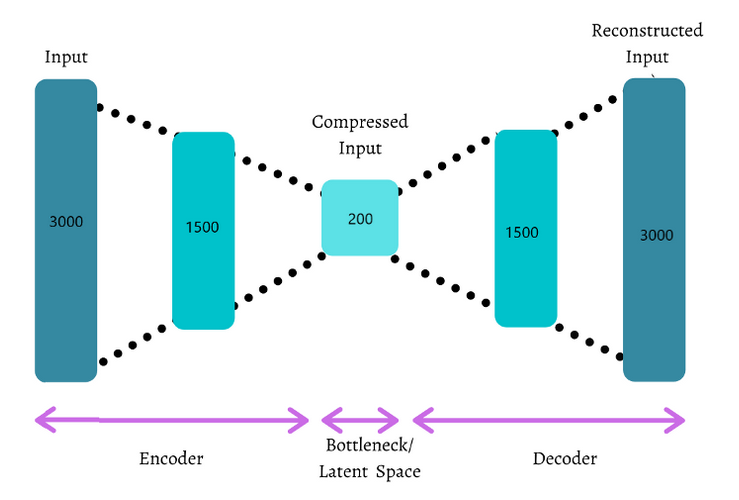
\includegraphics[width=\linewidth]{rys/dimensionality_reduction.png}
	\caption{Redukcja wymiarowości}
	\zrodlo{towards data science}
	\label{fig:dimensionality-reduction}
\end{figure}

Jak widać powyżej, autoenkoder składa się z trzech elementów:

Koder - funkcja służąca do kompresji danych do ich reprezentacji w niższym wymiarze.

Wąskie gardło - nazywane również przestrzenią ukrytą, gdzie nasze początkowe dane są reprezentowane w niższym wymiarze.

Dekoder - funkcja dekompresji lub rekonstrukcji danych o niskim wymiarze z powrotem do wymiaru początkowego.

Wymiar wejściowy i wymiar wyjściowy mają 3000 wymiarów, a pożądany wymiar zredukowany wynosi 200. Możemy stworzyć sieć pięciowarstwową, w której koder ma 3000 i 1500 neuronów, podobnie jak w przypadku sieci dekodera.

Embeddingi wektorowe skompresowanej warstwy wejściowej można traktować jako embedding warstwy wejściowej o zredukowanym wymiarze.

\subsection{Wyodrębnianie cech}

Autokodery mogą być używane jako ekstraktory cech w zadaniach klasyfikacji lub regresji. Autokodery pobierają nieoznakowane dane i uczą się efektywnych kodowań struktury danych, które mogą być wykorzystane w zadaniach uczenia nadzorowanego.

Po wytrenowaniu sieci auto-enkodera na próbce danych treningowych można zignorować część dekodera auto-enkodera, a jedynie użyć kodera do przekształcenia surowych danych wejściowych o wyższym wymiarze na przestrzeń zakodowaną o niższym wymiarze. Ten niższy wymiar danych może być wykorzystany jako cecha w zadaniach nadzorowanych.

\begin{figure}[!h]
	\centering
	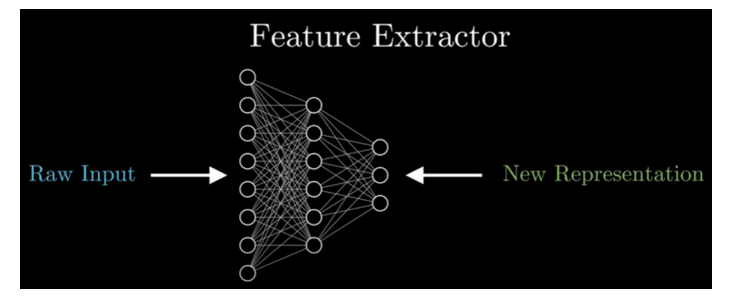
\includegraphics[width=\linewidth]{rys/feature_extractor.png}
	\caption{Wyodrębnianie cech}
	\zrodlo{towards data science}
	\label{fig:feature-extractor}
\end{figure}

\subsection{Odszumianie obrazów}

Surowe dane wejściowe ze świata rzeczywistego są często zaszumione, a wytrenowanie solidnego modelu nadzorowanego wymaga danych oczyszczonych i pozbawionych szumu. Do odszumiania danych można wykorzystać autoenkodery.

Jednym z popularnych zastosowań jest odszumianie obrazów, w którym autoenkodery próbują zrekonstruować obraz pozbawiony szumu z zaszumionego obrazu wejściowego.

\begin{figure}[!h]
	\centering
	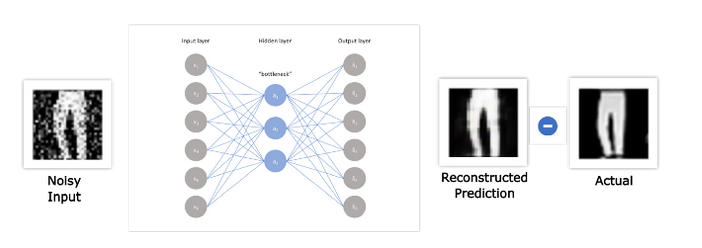
\includegraphics[width=\linewidth]{rys/image_denoising.png}
	\caption{Odszumianie obrazów}
	\zrodlo{towards data science}
	\label{fig:image-denoising}
\end{figure}

Zakłócony obraz wejściowy jest podawany do autoenkodera jako wejście, a bezszumowe wyjście jest rekonstruowane przez minimalizację straty rekonstrukcji w stosunku do oryginalnego wyjścia docelowego (bezszumowego). Po wytrenowaniu wag autoenkodera można je dalej wykorzystać do odszumiania obrazu surowego.

\subsection{Kompresja obrazu}

Innym zastosowaniem sieci auto-enkoderów jest kompresja obrazów. Surowy obraz wejściowy można przekazać do sieci kodera i uzyskać skompresowany wymiar zakodowanych danych. Wagi sieci autoenkodera mogą być uczone przez rekonstrukcję obrazu ze skompresowanego kodowania za pomocą sieci dekodera.

\begin{figure}[!h]
	\centering
	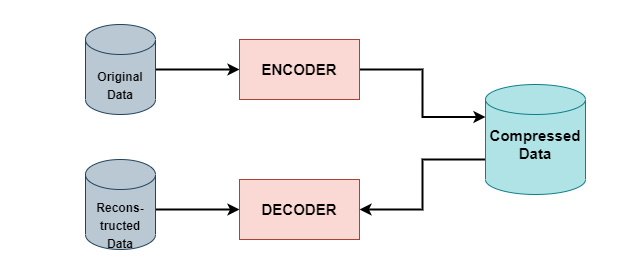
\includegraphics[width=\linewidth]{rys/image_compression.png}
	\caption{kompresja obrazów}
	\zrodlo{towards data science}
	\label{fig:image-compression}
\end{figure}

Zazwyczaj autoenkodery nie nadają się zbyt dobrze do kompresji danych, lepiej sprawdzają się raczej podstawowe algorytmy kompresji.

\subsection{Szukanie obrazu}

Do kompresji bazy danych obrazów można użyć autokoderów. Skompresowane osadzenie może być porównywane lub przeszukiwane z zakodowaną wersją szukanego obrazu.

\begin{figure}[!h]
	\centering
	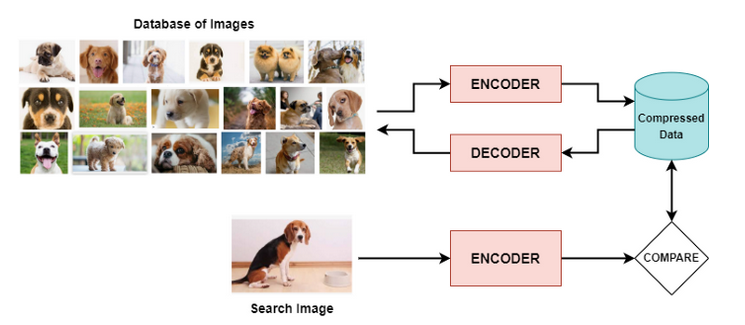
\includegraphics[width=\linewidth]{rys/image_search.png}
	\caption{szukanie obrazów}
	\zrodlo{towards data science}
	\label{fig:image-search}
\end{figure}

\subsection{Wykrywanie anomalii}

Innym użytecznym zastosowaniem sieci autoenkoderów jest wykrywanie anomalii. Model wykrywania anomalii można wykorzystać do wykrywania oszukańczych transakcji lub wszelkich zadań nadzorowanych o wysokim stopniu nierównowagi.

Idea polega na trenowaniu autoenkoderów tylko na próbkach danych jednej klasy (klasy większościowej). W ten sposób sieć jest w stanie zrekonstruować dane wejściowe z dobrą lub mniejszą stratą rekonstrukcji. Jeśli przez sieć autoenkodera przepuści się próbkę danych innej klasy docelowej, spowoduje to porównywalnie większą stratę rekonstrukcji.

Można określić wartość progową straty rekonstrukcji (wynik anomalii), której przekroczenie będzie uznawane za anomalię.

\subsection{Uzupełnianie brakujących danych}

Do imputacji brakujących wartości w zbiorze danych można wykorzystać autoenkodery odszumiające. Idea polega na trenowaniu sieci autoenkoderów poprzez losowe umieszczanie brakujących wartości w danych wejściowych i próbę odtworzenia oryginalnych danych surowych poprzez minimalizację straty rekonstrukcji.

Po wytrenowaniu wag autoenkodera rekordy zawierające brakujące wartości mogą być przepuszczane przez sieć autoenkodera w celu zrekonstruowania danych wejściowych, także z imputowanymi brakującymi cechami.



\chapter{Przykłady zastosowań autoenkoderów}

\section{Analiza PCA za pomocą autoenkodera niedopełnionego}

Jeśli autoenkoder korzysta jedynie z liniowych funkcji aktywacji, a funkcją kosztu jest  błąd średniokwadratowy (MSE), to będzie on przeprowadzał analizę składowych głównych PCA \cite{geron}. Na rysunku \ref{fig:PCA-kod} widoczny jest kod w języku Python służący do utworzenia takiego autoenkodera, który przeprowadzi analizę PCA na zbiorze trójwymiarowym, rzutując go na przestrzeń dwuwymiarową. Można zauważyć podział autoenkodera na dwie części - enkoder i dekoder. Enkoder przyjmuje dane wejściowe o wymiarze 3, a na wyjściu pojawiają się dane dwuwymiarowe. W przypadku dekodera jest odwrotnie - dane na wejściu są dwuwymiarowe, a na wyjściu trójwymiarowe. Obydwie części są modelami sekwencyjnymi z jedną warstwą gęstą, a cały autoenkoder jest modelem sekwencyjnym, w którym po enkoderze występuje dekoder.

\begin{figure}[!h]
	\centering
	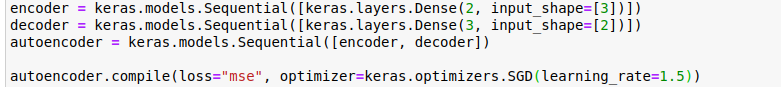
\includegraphics[width=\linewidth]{rys/autoenkoder_PCA_kod.png}
	\caption{Tworzenie autoenkodera niedopełnionego przeprowadzającego PCA}
	\zrodlo{Opracowanie własne na podstawie \cite{geron}}
	\label{fig:PCA-kod}
\end{figure}

\begin{figure}[!h]
	\centering
	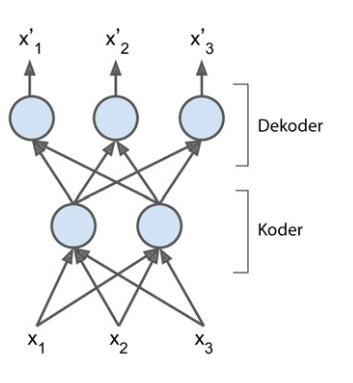
\includegraphics[width=7cm]{rys/ae_undercomplete.png}
	\caption{Architektura autoenkodera niedopełnionego}
	\zrodlo{\cite{geron}}
	\label{fig:ae-undercomplete}
\end{figure}

\newpage

Opisany autoenkoder zostanie wyuczony na wygenerowanym zbiorze trójwymiarowych danych. Warto zwrócić uwagę, że zbiór uczący stanowi jednocześnie dane wejściowe i dane docelowe. Po wytrenowaniu modelu, używamy enkodera do zakodowania danych wejściowych, czyli do zrzutowania ich na przestrzeń dwuwymiarową. Na rysunku \ref{fig:PCA-3d} zaprezentowany jest trójwymiarowy zbiór danych. Rysunek \ref{fig:PCA-2d} przedstawia wynik działania autoenkodera, a więc dane zrzutowane na przestrzeń 2D. Z kolei na rysunku \ref{fig:PCA-zwykle} widoczne jest rzutowanie uzyskane przy użyciu ,,zwykłego'' algorytmu PCA. Na podstawie tych wykresów można stwierdzić, że rzutowanie uzyskane przy pomocy autoenkodera oraz PCA jest takie samo, jedynie układ współrzędnych jest odwrócony o 180 stopni.

\newpage

\begin{figure}[!h]
	\centering
	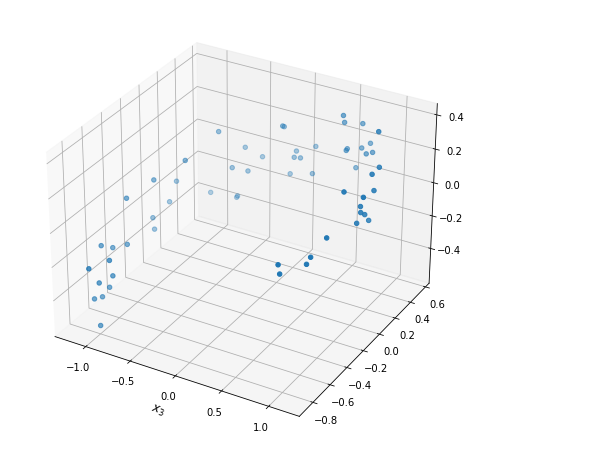
\includegraphics[width=10cm]{rys/pca3d_dane.png}
	\caption{Wygenerowane dane trójwymiarowe}
	\zrodlo{Opracowanie własne na podstawie \cite{geron}}
	\label{fig:PCA-3d}
\end{figure}


\begin{figure}[!h]
	\centering
	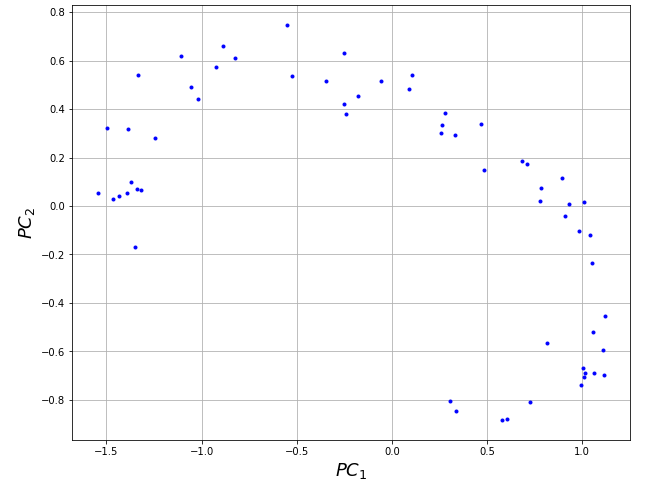
\includegraphics[width=10cm]{rys/pca2d_dane.png}
	\caption{Rzutowanie dwuwymiarowe przy użyciu autoenkodera, zachowujące maksymalną wariancję}
	\zrodlo{Opracowanie własne na podstawie \cite{geron}}
	\label{fig:PCA-2d}
\end{figure}

\newpage

\begin{figure}[!h]
	\centering
	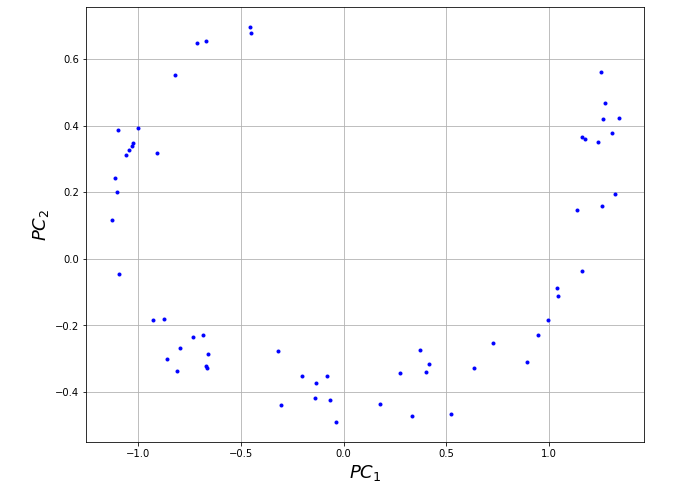
\includegraphics[width=10cm]{rys/pca_zwykle.png}
	\caption{Rzutowanie dwuwymiarowe przy użyciu PCA, zachowujące maksymalną wariancję}
	\zrodlo{Opracowanie własne na podstawie \cite{geron}}
	\label{fig:PCA-zwykle}
\end{figure}

\begin{figure}[!h]
	\centering
	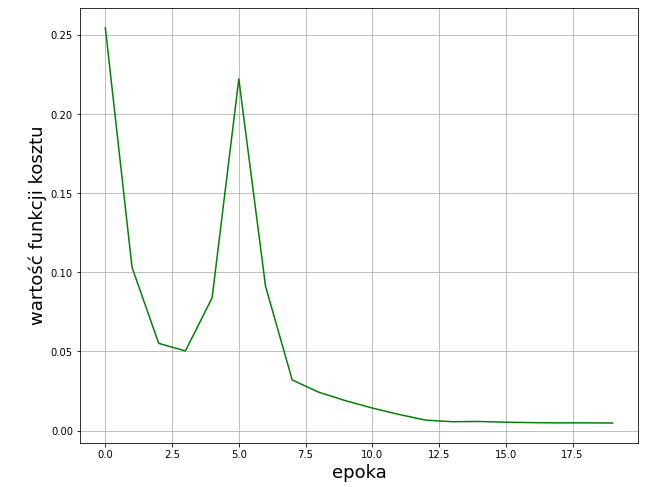
\includegraphics[width=10cm]{rys/ae_undercomplete_loss.png}
	\caption{Wartość funkcji straty w kolejnych epokach podczas uczenia modelu}
	\zrodlo{Opracowanie własne}
	\label{fig:undercomplete-loss}
\end{figure}

\section{Kolejny przykład}


\chapter*{Podsumowanie i~wnioski}


\begin{thebibliography}{99}

\bibitem{aggarwal} Aggarwal, C. C. (2018).\emph{ Neural Networks and Deep Learning}, Springer International Publishing

\bibitem{bank} Bank D., Koenigstein N., Giryes R. (2021), \emph{Autoencoders}, arXiv:2003.05991v2

\bibitem{chollet} Chollet F., Allaire J. J. (2019) \emph{Deep Learning. Praca z językiem R i biblioteką Keras}, Helion SA

\bibitem{edureka} Edureka, Autoencoders Tutorial. Autoencoders in Deep Learning. Tensorflow Training \url{https://www.youtube.com/watch?v=nTt_ajul8NY} 

\bibitem{ertel} Ertel W. (2017) \emph{Introduction to Artificial Intelligence. Second Edition}, Springer International Publishing

\bibitem{geron} G\'eron A. (2020) \emph{Uczenie maszynowe z użyciem Scikit-Learn i TensorFlow. Wydanie II}, Helion SA

\bibitem{goodfellow} Goodfellow I., Bengio Y., Courville A. (2018), \emph{Deep Learning. Systemy uczące się}, PWN, Warszawa 

\bibitem{illustrated} Krohn J., Beyleveld G., Bassens A., \emph{Uczenie głębokie i sztuczna inteligencja. Interaktywny przewodnik ilustrowany}, Helion 2022

\bibitem{osinga} Osinga D. (2019) \emph{Deep Learning. Receptury}, Helion SA

\bibitem{skansi} Skansi S. (2018) \emph{Introduction to Deep Learning. From Logical Calculus to Artificial Intelligence}, Springer International Publishing


\end{thebibliography}



\listoffigures

\listoftables


\chapter*{Załączniki}
\begin{enumerate}
%\item Oświadczenie o oryginalności pracy i możliwości jej wykorzystania. 
%\item Opinia promotora na temat oryginalności pracy oraz w~sprawie dopuszczenia do obrony pracy dyplomowej.
%\item Potwierdzenie analizy antyplagiatowej.
\item Płyta CD z niniejszą pracą w wersji elektronicznej.
\end{enumerate}




\chapter*{Streszczenie (Summary)}

\bigskip
\bigskip

\begin{center}
  \textbf{\tytul}
\end{center}



\bigskip

\begin{center}
  \textbf{\textit{\tytulangielski}}
\end{center}



\selecthyphenation{english}
{\it

}

\end{document}

